\documentclass[sigconf]{acmart}

\settopmatter{printacmref=false}
\setcopyright{none}
\renewcommand\footnotetextcopyrightpermission[1]{}
\acmConference[CS6215 Fall 2026]{CS6215 Advanced Topics in Program Analysis, Individual Course Project}{Fall 2026}{National University of Singapore}
\acmYear{2026}
\acmDOI{}
\acmISBN{}

\usepackage{enumitem}
\usepackage{xspace}
\usepackage{url}
\DeclareUrlCommand\code{\urlstyle{tt}}
\setlength{\emergencystretch}{1.5em}
\raggedbottom
% A highlighted answer box at the end of each research question.
\newcommand{\answer}[2]{\par\smallskip\noindent\fcolorbox{black!40}{black!5}{\parbox{\dimexpr\linewidth-2\fboxsep-2\fboxrule\relax}{\small\textbf{Answer to #1.} #2}}\par\smallskip}
\newcommand{\nscg}{NSCG\xspace}
% generated by eval/tables.py; use \R{key}
\makeatletter
\expandafter\def\csname res@autojump-in-f1-inter--pycg-2026--nscg-v21\endcsname{1.000}
\expandafter\def\csname res@autojump-in-f1-llm-only\endcsname{1.000}
\expandafter\def\csname res@autojump-in-f1-llm-only@sonnet\endcsname{0.944}
\expandafter\def\csname res@autojump-in-f1-nscg\endcsname{1.000}
\expandafter\def\csname res@autojump-in-f1-nscg-hybrid\endcsname{0.939}
\expandafter\def\csname res@autojump-in-f1-nscg-hybrid-v21\endcsname{0.939}
\expandafter\def\csname res@autojump-in-f1-nscg-nohints\endcsname{1.000}
\expandafter\def\csname res@autojump-in-f1-nscg-sym\endcsname{0.939}
\expandafter\def\csname res@autojump-in-f1-nscg-v21\endcsname{1.000}
\expandafter\def\csname res@autojump-in-f1-nscg-v21-r1\endcsname{1.000}
\expandafter\def\csname res@autojump-in-f1-nscg-v21-r2\endcsname{1.000}
\expandafter\def\csname res@autojump-in-f1-nscg-v21@sonnet\endcsname{0.946}
\expandafter\def\csname res@autojump-in-f1-pycg-2021\endcsname{0.939}
\expandafter\def\csname res@autojump-in-f1-pycg-2026\endcsname{0.946}
\expandafter\def\csname res@autojump-in-f1-union--pycg-2026--nscg-v21\endcsname{0.946}
\expandafter\def\csname res@autojump-in-fn-inter--pycg-2026--nscg-v21\endcsname{0}
\expandafter\def\csname res@autojump-in-fn-llm-only\endcsname{0}
\expandafter\def\csname res@autojump-in-fn-llm-only@sonnet\endcsname{1}
\expandafter\def\csname res@autojump-in-fn-nscg\endcsname{0}
\expandafter\def\csname res@autojump-in-fn-nscg-hybrid\endcsname{4}
\expandafter\def\csname res@autojump-in-fn-nscg-hybrid-v21\endcsname{4}
\expandafter\def\csname res@autojump-in-fn-nscg-nohints\endcsname{0}
\expandafter\def\csname res@autojump-in-fn-nscg-sym\endcsname{4}
\expandafter\def\csname res@autojump-in-fn-nscg-v21\endcsname{0}
\expandafter\def\csname res@autojump-in-fn-nscg-v21-r1\endcsname{0}
\expandafter\def\csname res@autojump-in-fn-nscg-v21-r2\endcsname{0}
\expandafter\def\csname res@autojump-in-fn-nscg-v21@sonnet\endcsname{0}
\expandafter\def\csname res@autojump-in-fn-pycg-2021\endcsname{4}
\expandafter\def\csname res@autojump-in-fn-pycg-2026\endcsname{0}
\expandafter\def\csname res@autojump-in-fn-union--pycg-2026--nscg-v21\endcsname{0}
\expandafter\def\csname res@autojump-in-fp-inter--pycg-2026--nscg-v21\endcsname{0}
\expandafter\def\csname res@autojump-in-fp-llm-only\endcsname{0}
\expandafter\def\csname res@autojump-in-fp-llm-only@sonnet\endcsname{3}
\expandafter\def\csname res@autojump-in-fp-nscg\endcsname{0}
\expandafter\def\csname res@autojump-in-fp-nscg-hybrid\endcsname{0}
\expandafter\def\csname res@autojump-in-fp-nscg-hybrid-v21\endcsname{0}
\expandafter\def\csname res@autojump-in-fp-nscg-nohints\endcsname{0}
\expandafter\def\csname res@autojump-in-fp-nscg-sym\endcsname{0}
\expandafter\def\csname res@autojump-in-fp-nscg-v21\endcsname{0}
\expandafter\def\csname res@autojump-in-fp-nscg-v21-r1\endcsname{0}
\expandafter\def\csname res@autojump-in-fp-nscg-v21-r2\endcsname{0}
\expandafter\def\csname res@autojump-in-fp-nscg-v21@sonnet\endcsname{4}
\expandafter\def\csname res@autojump-in-fp-pycg-2021\endcsname{0}
\expandafter\def\csname res@autojump-in-fp-pycg-2026\endcsname{4}
\expandafter\def\csname res@autojump-in-fp-union--pycg-2026--nscg-v21\endcsname{4}
\expandafter\def\csname res@autojump-in-p-inter--pycg-2026--nscg-v21\endcsname{1.000}
\expandafter\def\csname res@autojump-in-p-llm-only\endcsname{1.000}
\expandafter\def\csname res@autojump-in-p-llm-only@sonnet\endcsname{0.919}
\expandafter\def\csname res@autojump-in-p-nscg\endcsname{1.000}
\expandafter\def\csname res@autojump-in-p-nscg-hybrid\endcsname{1.000}
\expandafter\def\csname res@autojump-in-p-nscg-hybrid-v21\endcsname{1.000}
\expandafter\def\csname res@autojump-in-p-nscg-nohints\endcsname{1.000}
\expandafter\def\csname res@autojump-in-p-nscg-sym\endcsname{1.000}
\expandafter\def\csname res@autojump-in-p-nscg-v21\endcsname{1.000}
\expandafter\def\csname res@autojump-in-p-nscg-v21-r1\endcsname{1.000}
\expandafter\def\csname res@autojump-in-p-nscg-v21-r2\endcsname{1.000}
\expandafter\def\csname res@autojump-in-p-nscg-v21@sonnet\endcsname{0.897}
\expandafter\def\csname res@autojump-in-p-pycg-2021\endcsname{1.000}
\expandafter\def\csname res@autojump-in-p-pycg-2026\endcsname{0.897}
\expandafter\def\csname res@autojump-in-p-union--pycg-2026--nscg-v21\endcsname{0.897}
\expandafter\def\csname res@autojump-in-r-inter--pycg-2026--nscg-v21\endcsname{1.000}
\expandafter\def\csname res@autojump-in-r-llm-only\endcsname{1.000}
\expandafter\def\csname res@autojump-in-r-llm-only@sonnet\endcsname{0.971}
\expandafter\def\csname res@autojump-in-r-nscg\endcsname{1.000}
\expandafter\def\csname res@autojump-in-r-nscg-hybrid\endcsname{0.886}
\expandafter\def\csname res@autojump-in-r-nscg-hybrid-v21\endcsname{0.886}
\expandafter\def\csname res@autojump-in-r-nscg-nohints\endcsname{1.000}
\expandafter\def\csname res@autojump-in-r-nscg-sym\endcsname{0.886}
\expandafter\def\csname res@autojump-in-r-nscg-v21\endcsname{1.000}
\expandafter\def\csname res@autojump-in-r-nscg-v21-r1\endcsname{1.000}
\expandafter\def\csname res@autojump-in-r-nscg-v21-r2\endcsname{1.000}
\expandafter\def\csname res@autojump-in-r-nscg-v21@sonnet\endcsname{1.000}
\expandafter\def\csname res@autojump-in-r-pycg-2021\endcsname{0.886}
\expandafter\def\csname res@autojump-in-r-pycg-2026\endcsname{1.000}
\expandafter\def\csname res@autojump-in-r-union--pycg-2026--nscg-v21\endcsname{1.000}
\expandafter\def\csname res@autojump-status-inter--pycg-2026--nscg-v21\endcsname{ok}
\expandafter\def\csname res@autojump-status-llm-only\endcsname{ok}
\expandafter\def\csname res@autojump-status-llm-only@sonnet\endcsname{ok}
\expandafter\def\csname res@autojump-status-nscg\endcsname{ok}
\expandafter\def\csname res@autojump-status-nscg-hybrid\endcsname{ok}
\expandafter\def\csname res@autojump-status-nscg-hybrid-v21\endcsname{ok}
\expandafter\def\csname res@autojump-status-nscg-nohints\endcsname{ok}
\expandafter\def\csname res@autojump-status-nscg-sym\endcsname{ok}
\expandafter\def\csname res@autojump-status-nscg-v21\endcsname{ok}
\expandafter\def\csname res@autojump-status-nscg-v21-r1\endcsname{ok}
\expandafter\def\csname res@autojump-status-nscg-v21-r2\endcsname{ok}
\expandafter\def\csname res@autojump-status-nscg-v21@sonnet\endcsname{ok}
\expandafter\def\csname res@autojump-status-pycg-2021\endcsname{ok}
\expandafter\def\csname res@autojump-status-pycg-2026\endcsname{ok}
\expandafter\def\csname res@autojump-status-union--pycg-2026--nscg-v21\endcsname{ok}
\expandafter\def\csname res@err-fn-ext-misnamed-llm-only\endcsname{24}
\expandafter\def\csname res@err-fn-ext-misnamed-nscg\endcsname{64}
\expandafter\def\csname res@err-fn-ext-misnamed-nscg-hybrid-v21\endcsname{53}
\expandafter\def\csname res@err-fn-ext-misnamed-nscg-nohints\endcsname{46}
\expandafter\def\csname res@err-fn-ext-misnamed-nscg-sym\endcsname{56}
\expandafter\def\csname res@err-fn-ext-misnamed-nscg-v21\endcsname{53}
\expandafter\def\csname res@err-fn-ext-omitted-llm-only\endcsname{199}
\expandafter\def\csname res@err-fn-ext-omitted-nscg\endcsname{82}
\expandafter\def\csname res@err-fn-ext-omitted-nscg-hybrid-v21\endcsname{66}
\expandafter\def\csname res@err-fn-ext-omitted-nscg-nohints\endcsname{119}
\expandafter\def\csname res@err-fn-ext-omitted-nscg-sym\endcsname{215}
\expandafter\def\csname res@err-fn-ext-omitted-nscg-v21\endcsname{80}
\expandafter\def\csname res@err-fn-no-evidence-llm-only\endcsname{276}
\expandafter\def\csname res@err-fn-no-evidence-nscg\endcsname{255}
\expandafter\def\csname res@err-fn-no-evidence-nscg-hybrid-v21\endcsname{253}
\expandafter\def\csname res@err-fn-no-evidence-nscg-nohints\endcsname{260}
\expandafter\def\csname res@err-fn-no-evidence-nscg-sym\endcsname{389}
\expandafter\def\csname res@err-fn-no-evidence-nscg-v21\endcsname{253}
\expandafter\def\csname res@err-fn-rejected-llm-only\endcsname{25}
\expandafter\def\csname res@err-fn-rejected-nscg\endcsname{3}
\expandafter\def\csname res@err-fn-rejected-nscg-hybrid-v21\endcsname{6}
\expandafter\def\csname res@err-fn-rejected-nscg-nohints\endcsname{24}
\expandafter\def\csname res@err-fn-rejected-nscg-sym\endcsname{41}
\expandafter\def\csname res@err-fn-rejected-nscg-v21\endcsname{3}
\expandafter\def\csname res@err-fp-accepted-hint-llm-only\endcsname{16}
\expandafter\def\csname res@err-fp-accepted-hint-nscg\endcsname{57}
\expandafter\def\csname res@err-fp-accepted-hint-nscg-hybrid-v21\endcsname{53}
\expandafter\def\csname res@err-fp-accepted-hint-nscg-nohints\endcsname{18}
\expandafter\def\csname res@err-fp-accepted-hint-nscg-sym\endcsname{20}
\expandafter\def\csname res@err-fp-accepted-hint-nscg-v21\endcsname{57}
\expandafter\def\csname res@err-fp-ext-misnamed-llm-only\endcsname{10}
\expandafter\def\csname res@err-fp-ext-misnamed-nscg\endcsname{61}
\expandafter\def\csname res@err-fp-ext-misnamed-nscg-hybrid-v21\endcsname{41}
\expandafter\def\csname res@err-fp-ext-misnamed-nscg-nohints\endcsname{44}
\expandafter\def\csname res@err-fp-ext-misnamed-nscg-sym\endcsname{63}
\expandafter\def\csname res@err-fp-ext-misnamed-nscg-v21\endcsname{43}
\expandafter\def\csname res@err-fp-ext-spurious-llm-only\endcsname{16}
\expandafter\def\csname res@err-fp-ext-spurious-nscg\endcsname{48}
\expandafter\def\csname res@err-fp-ext-spurious-nscg-hybrid-v21\endcsname{34}
\expandafter\def\csname res@err-fp-ext-spurious-nscg-nohints\endcsname{29}
\expandafter\def\csname res@err-fp-ext-spurious-nscg-sym\endcsname{20}
\expandafter\def\csname res@err-fp-ext-spurious-nscg-v21\endcsname{48}
\expandafter\def\csname res@err-fp-llm-added-llm-only\endcsname{13}
\expandafter\def\csname res@err-fp-llm-added-nscg\endcsname{10}
\expandafter\def\csname res@err-fp-llm-added-nscg-hybrid-v21\endcsname{5}
\expandafter\def\csname res@err-fp-llm-added-nscg-nohints\endcsname{5}
\expandafter\def\csname res@err-fp-llm-added-nscg-v21\endcsname{10}
\expandafter\def\csname res@fabric-in-f1-inter--pycg-2026--nscg-v21\endcsname{0.705}
\expandafter\def\csname res@fabric-in-f1-llm-only\endcsname{0.709}
\expandafter\def\csname res@fabric-in-f1-llm-only@sonnet\endcsname{0.651}
\expandafter\def\csname res@fabric-in-f1-nscg\endcsname{0.726}
\expandafter\def\csname res@fabric-in-f1-nscg-hybrid\endcsname{0.741}
\expandafter\def\csname res@fabric-in-f1-nscg-hybrid-v21\endcsname{0.741}
\expandafter\def\csname res@fabric-in-f1-nscg-nohints\endcsname{0.741}
\expandafter\def\csname res@fabric-in-f1-nscg-sym\endcsname{0.635}
\expandafter\def\csname res@fabric-in-f1-nscg-v21\endcsname{0.741}
\expandafter\def\csname res@fabric-in-f1-nscg-v21-r1\endcsname{0.741}
\expandafter\def\csname res@fabric-in-f1-nscg-v21-r2\endcsname{0.741}
\expandafter\def\csname res@fabric-in-f1-nscg-v21@sonnet\endcsname{0.820}
\expandafter\def\csname res@fabric-in-f1-pycg-2021\endcsname{0.617}
\expandafter\def\csname res@fabric-in-f1-pycg-2026\endcsname{0.705}
\expandafter\def\csname res@fabric-in-f1-union--pycg-2026--nscg-v21\endcsname{0.741}
\expandafter\def\csname res@fabric-in-fn-inter--pycg-2026--nscg-v21\endcsname{44}
\expandafter\def\csname res@fabric-in-fn-llm-only\endcsname{38}
\expandafter\def\csname res@fabric-in-fn-llm-only@sonnet\endcsname{43}
\expandafter\def\csname res@fabric-in-fn-nscg\endcsname{38}
\expandafter\def\csname res@fabric-in-fn-nscg-hybrid\endcsname{36}
\expandafter\def\csname res@fabric-in-fn-nscg-hybrid-v21\endcsname{36}
\expandafter\def\csname res@fabric-in-fn-nscg-nohints\endcsname{36}
\expandafter\def\csname res@fabric-in-fn-nscg-sym\endcsname{52}
\expandafter\def\csname res@fabric-in-fn-nscg-v21\endcsname{36}
\expandafter\def\csname res@fabric-in-fn-nscg-v21-r1\endcsname{36}
\expandafter\def\csname res@fabric-in-fn-nscg-v21-r2\endcsname{36}
\expandafter\def\csname res@fabric-in-fn-nscg-v21@sonnet\endcsname{24}
\expandafter\def\csname res@fabric-in-fn-pycg-2021\endcsname{53}
\expandafter\def\csname res@fabric-in-fn-pycg-2026\endcsname{44}
\expandafter\def\csname res@fabric-in-fn-union--pycg-2026--nscg-v21\endcsname{36}
\expandafter\def\csname res@fabric-in-fp-inter--pycg-2026--nscg-v21\endcsname{2}
\expandafter\def\csname res@fabric-in-fp-llm-only\endcsname{12}
\expandafter\def\csname res@fabric-in-fp-llm-only@sonnet\endcsname{17}
\expandafter\def\csname res@fabric-in-fp-nscg\endcsname{8}
\expandafter\def\csname res@fabric-in-fp-nscg-hybrid\endcsname{8}
\expandafter\def\csname res@fabric-in-fp-nscg-hybrid-v21\endcsname{8}
\expandafter\def\csname res@fabric-in-fp-nscg-nohints\endcsname{8}
\expandafter\def\csname res@fabric-in-fp-nscg-sym\endcsname{2}
\expandafter\def\csname res@fabric-in-fp-nscg-v21\endcsname{8}
\expandafter\def\csname res@fabric-in-fp-nscg-v21-r1\endcsname{8}
\expandafter\def\csname res@fabric-in-fp-nscg-v21-r2\endcsname{8}
\expandafter\def\csname res@fabric-in-fp-nscg-v21@sonnet\endcsname{9}
\expandafter\def\csname res@fabric-in-fp-pycg-2021\endcsname{4}
\expandafter\def\csname res@fabric-in-fp-pycg-2026\endcsname{2}
\expandafter\def\csname res@fabric-in-fp-union--pycg-2026--nscg-v21\endcsname{8}
\expandafter\def\csname res@fabric-in-p-inter--pycg-2026--nscg-v21\endcsname{0.965}
\expandafter\def\csname res@fabric-in-p-llm-only\endcsname{0.836}
\expandafter\def\csname res@fabric-in-p-llm-only@sonnet\endcsname{0.767}
\expandafter\def\csname res@fabric-in-p-nscg\endcsname{0.884}
\expandafter\def\csname res@fabric-in-p-nscg-hybrid\endcsname{0.887}
\expandafter\def\csname res@fabric-in-p-nscg-hybrid-v21\endcsname{0.887}
\expandafter\def\csname res@fabric-in-p-nscg-nohints\endcsname{0.887}
\expandafter\def\csname res@fabric-in-p-nscg-sym\endcsname{0.959}
\expandafter\def\csname res@fabric-in-p-nscg-v21\endcsname{0.887}
\expandafter\def\csname res@fabric-in-p-nscg-v21-r1\endcsname{0.887}
\expandafter\def\csname res@fabric-in-p-nscg-v21-r2\endcsname{0.887}
\expandafter\def\csname res@fabric-in-p-nscg-v21@sonnet\endcsname{0.893}
\expandafter\def\csname res@fabric-in-p-pycg-2021\endcsname{0.920}
\expandafter\def\csname res@fabric-in-p-pycg-2026\endcsname{0.965}
\expandafter\def\csname res@fabric-in-p-union--pycg-2026--nscg-v21\endcsname{0.887}
\expandafter\def\csname res@fabric-in-r-inter--pycg-2026--nscg-v21\endcsname{0.556}
\expandafter\def\csname res@fabric-in-r-llm-only\endcsname{0.616}
\expandafter\def\csname res@fabric-in-r-llm-only@sonnet\endcsname{0.566}
\expandafter\def\csname res@fabric-in-r-nscg\endcsname{0.616}
\expandafter\def\csname res@fabric-in-r-nscg-hybrid\endcsname{0.636}
\expandafter\def\csname res@fabric-in-r-nscg-hybrid-v21\endcsname{0.636}
\expandafter\def\csname res@fabric-in-r-nscg-nohints\endcsname{0.636}
\expandafter\def\csname res@fabric-in-r-nscg-sym\endcsname{0.475}
\expandafter\def\csname res@fabric-in-r-nscg-v21\endcsname{0.636}
\expandafter\def\csname res@fabric-in-r-nscg-v21-r1\endcsname{0.636}
\expandafter\def\csname res@fabric-in-r-nscg-v21-r2\endcsname{0.636}
\expandafter\def\csname res@fabric-in-r-nscg-v21@sonnet\endcsname{0.758}
\expandafter\def\csname res@fabric-in-r-pycg-2021\endcsname{0.465}
\expandafter\def\csname res@fabric-in-r-pycg-2026\endcsname{0.556}
\expandafter\def\csname res@fabric-in-r-union--pycg-2026--nscg-v21\endcsname{0.636}
\expandafter\def\csname res@fabric-status-inter--pycg-2026--nscg-v21\endcsname{ok}
\expandafter\def\csname res@fabric-status-llm-only\endcsname{ok}
\expandafter\def\csname res@fabric-status-llm-only@sonnet\endcsname{ok}
\expandafter\def\csname res@fabric-status-nscg\endcsname{ok}
\expandafter\def\csname res@fabric-status-nscg-hybrid\endcsname{ok}
\expandafter\def\csname res@fabric-status-nscg-hybrid-v21\endcsname{ok}
\expandafter\def\csname res@fabric-status-nscg-nohints\endcsname{ok}
\expandafter\def\csname res@fabric-status-nscg-sym\endcsname{ok}
\expandafter\def\csname res@fabric-status-nscg-v21\endcsname{ok}
\expandafter\def\csname res@fabric-status-nscg-v21-r1\endcsname{ok}
\expandafter\def\csname res@fabric-status-nscg-v21-r2\endcsname{ok}
\expandafter\def\csname res@fabric-status-nscg-v21@sonnet\endcsname{ok}
\expandafter\def\csname res@fabric-status-pycg-2021\endcsname{ok}
\expandafter\def\csname res@fabric-status-pycg-2026\endcsname{ok}
\expandafter\def\csname res@fabric-status-union--pycg-2026--nscg-v21\endcsname{ok}
\expandafter\def\csname res@funcy-in-f1-inter--pycg-2026--nscg-v21\endcsname{0.678}
\expandafter\def\csname res@funcy-in-f1-llm-only\endcsname{0.639}
\expandafter\def\csname res@funcy-in-f1-llm-only@sonnet\endcsname{0.648}
\expandafter\def\csname res@funcy-in-f1-nscg\endcsname{0.680}
\expandafter\def\csname res@funcy-in-f1-nscg-hybrid\endcsname{0.687}
\expandafter\def\csname res@funcy-in-f1-nscg-hybrid-v21\endcsname{0.687}
\expandafter\def\csname res@funcy-in-f1-nscg-nohints\endcsname{0.669}
\expandafter\def\csname res@funcy-in-f1-nscg-sym\endcsname{0.597}
\expandafter\def\csname res@funcy-in-f1-nscg-v21\endcsname{0.680}
\expandafter\def\csname res@funcy-in-f1-nscg-v21-r1\endcsname{0.665}
\expandafter\def\csname res@funcy-in-f1-nscg-v21-r2\endcsname{0.694}
\expandafter\def\csname res@funcy-in-f1-nscg-v21@sonnet\endcsname{0.685}
\expandafter\def\csname res@funcy-in-f1-pycg-2021\endcsname{--}
\expandafter\def\csname res@funcy-in-f1-pycg-2026\endcsname{0.654}
\expandafter\def\csname res@funcy-in-f1-union--pycg-2026--nscg-v21\endcsname{0.657}
\expandafter\def\csname res@funcy-in-fn-inter--pycg-2026--nscg-v21\endcsname{242}
\expandafter\def\csname res@funcy-in-fn-llm-only\endcsname{263}
\expandafter\def\csname res@funcy-in-fn-llm-only@sonnet\endcsname{262}
\expandafter\def\csname res@funcy-in-fn-nscg\endcsname{218}
\expandafter\def\csname res@funcy-in-fn-nscg-hybrid\endcsname{218}
\expandafter\def\csname res@funcy-in-fn-nscg-hybrid-v21\endcsname{218}
\expandafter\def\csname res@funcy-in-fn-nscg-nohints\endcsname{247}
\expandafter\def\csname res@funcy-in-fn-nscg-sym\endcsname{286}
\expandafter\def\csname res@funcy-in-fn-nscg-v21\endcsname{218}
\expandafter\def\csname res@funcy-in-fn-nscg-v21-r1\endcsname{218}
\expandafter\def\csname res@funcy-in-fn-nscg-v21-r2\endcsname{219}
\expandafter\def\csname res@funcy-in-fn-nscg-v21@sonnet\endcsname{224}
\expandafter\def\csname res@funcy-in-fn-pycg-2021\endcsname{511}
\expandafter\def\csname res@funcy-in-fn-pycg-2026\endcsname{230}
\expandafter\def\csname res@funcy-in-fn-union--pycg-2026--nscg-v21\endcsname{206}
\expandafter\def\csname res@funcy-in-fp-inter--pycg-2026--nscg-v21\endcsname{13}
\expandafter\def\csname res@funcy-in-fp-llm-only\endcsname{17}
\expandafter\def\csname res@funcy-in-fp-llm-only@sonnet\endcsname{9}
\expandafter\def\csname res@funcy-in-fp-nscg\endcsname{58}
\expandafter\def\csname res@funcy-in-fp-nscg-hybrid\endcsname{49}
\expandafter\def\csname res@funcy-in-fp-nscg-hybrid-v21\endcsname{49}
\expandafter\def\csname res@funcy-in-fp-nscg-nohints\endcsname{14}
\expandafter\def\csname res@funcy-in-fp-nscg-sym\endcsname{18}
\expandafter\def\csname res@funcy-in-fp-nscg-v21\endcsname{58}
\expandafter\def\csname res@funcy-in-fp-nscg-v21-r1\endcsname{77}
\expandafter\def\csname res@funcy-in-fp-nscg-v21-r2\endcsname{39}
\expandafter\def\csname res@funcy-in-fp-nscg-v21@sonnet\endcsname{40}
\expandafter\def\csname res@funcy-in-fp-pycg-2021\endcsname{0}
\expandafter\def\csname res@funcy-in-fp-pycg-2026\endcsname{67}
\expandafter\def\csname res@funcy-in-fp-union--pycg-2026--nscg-v21\endcsname{112}
\expandafter\def\csname res@funcy-in-p-inter--pycg-2026--nscg-v21\endcsname{0.954}
\expandafter\def\csname res@funcy-in-p-llm-only\endcsname{0.936}
\expandafter\def\csname res@funcy-in-p-llm-only@sonnet\endcsname{0.965}
\expandafter\def\csname res@funcy-in-p-nscg\endcsname{0.835}
\expandafter\def\csname res@funcy-in-p-nscg-hybrid\endcsname{0.857}
\expandafter\def\csname res@funcy-in-p-nscg-hybrid-v21\endcsname{0.857}
\expandafter\def\csname res@funcy-in-p-nscg-nohints\endcsname{0.950}
\expandafter\def\csname res@funcy-in-p-nscg-sym\endcsname{0.926}
\expandafter\def\csname res@funcy-in-p-nscg-v21\endcsname{0.835}
\expandafter\def\csname res@funcy-in-p-nscg-v21-r1\endcsname{0.792}
\expandafter\def\csname res@funcy-in-p-nscg-v21-r2\endcsname{0.882}
\expandafter\def\csname res@funcy-in-p-nscg-v21@sonnet\endcsname{0.878}
\expandafter\def\csname res@funcy-in-p-pycg-2021\endcsname{--}
\expandafter\def\csname res@funcy-in-p-pycg-2026\endcsname{0.807}
\expandafter\def\csname res@funcy-in-p-union--pycg-2026--nscg-v21\endcsname{0.731}
\expandafter\def\csname res@funcy-in-r-inter--pycg-2026--nscg-v21\endcsname{0.526}
\expandafter\def\csname res@funcy-in-r-llm-only\endcsname{0.485}
\expandafter\def\csname res@funcy-in-r-llm-only@sonnet\endcsname{0.487}
\expandafter\def\csname res@funcy-in-r-nscg\endcsname{0.573}
\expandafter\def\csname res@funcy-in-r-nscg-hybrid\endcsname{0.573}
\expandafter\def\csname res@funcy-in-r-nscg-hybrid-v21\endcsname{0.573}
\expandafter\def\csname res@funcy-in-r-nscg-nohints\endcsname{0.517}
\expandafter\def\csname res@funcy-in-r-nscg-sym\endcsname{0.440}
\expandafter\def\csname res@funcy-in-r-nscg-v21\endcsname{0.573}
\expandafter\def\csname res@funcy-in-r-nscg-v21-r1\endcsname{0.573}
\expandafter\def\csname res@funcy-in-r-nscg-v21-r2\endcsname{0.571}
\expandafter\def\csname res@funcy-in-r-nscg-v21@sonnet\endcsname{0.562}
\expandafter\def\csname res@funcy-in-r-pycg-2021\endcsname{0.000}
\expandafter\def\csname res@funcy-in-r-pycg-2026\endcsname{0.550}
\expandafter\def\csname res@funcy-in-r-union--pycg-2026--nscg-v21\endcsname{0.597}
\expandafter\def\csname res@funcy-status-inter--pycg-2026--nscg-v21\endcsname{ok}
\expandafter\def\csname res@funcy-status-llm-only\endcsname{ok}
\expandafter\def\csname res@funcy-status-llm-only@sonnet\endcsname{ok}
\expandafter\def\csname res@funcy-status-nscg\endcsname{ok}
\expandafter\def\csname res@funcy-status-nscg-hybrid\endcsname{ok}
\expandafter\def\csname res@funcy-status-nscg-hybrid-v21\endcsname{ok}
\expandafter\def\csname res@funcy-status-nscg-nohints\endcsname{ok}
\expandafter\def\csname res@funcy-status-nscg-sym\endcsname{ok}
\expandafter\def\csname res@funcy-status-nscg-v21\endcsname{ok}
\expandafter\def\csname res@funcy-status-nscg-v21-r1\endcsname{ok}
\expandafter\def\csname res@funcy-status-nscg-v21-r2\endcsname{ok}
\expandafter\def\csname res@funcy-status-nscg-v21@sonnet\endcsname{ok}
\expandafter\def\csname res@funcy-status-pycg-2021\endcsname{timeout}
\expandafter\def\csname res@funcy-status-pycg-2026\endcsname{ok}
\expandafter\def\csname res@funcy-status-union--pycg-2026--nscg-v21\endcsname{ok}
\expandafter\def\csname res@jmespath-in-f1-inter--pycg-2026--nscg-v21\endcsname{0.995}
\expandafter\def\csname res@jmespath-in-f1-llm-only\endcsname{1.000}
\expandafter\def\csname res@jmespath-in-f1-llm-only@sonnet\endcsname{0.887}
\expandafter\def\csname res@jmespath-in-f1-nscg\endcsname{0.995}
\expandafter\def\csname res@jmespath-in-f1-nscg-hybrid\endcsname{0.997}
\expandafter\def\csname res@jmespath-in-f1-nscg-hybrid-v21\endcsname{0.997}
\expandafter\def\csname res@jmespath-in-f1-nscg-nohints\endcsname{0.997}
\expandafter\def\csname res@jmespath-in-f1-nscg-sym\endcsname{0.835}
\expandafter\def\csname res@jmespath-in-f1-nscg-v21\endcsname{0.995}
\expandafter\def\csname res@jmespath-in-f1-nscg-v21-r1\endcsname{0.995}
\expandafter\def\csname res@jmespath-in-f1-nscg-v21-r2\endcsname{0.997}
\expandafter\def\csname res@jmespath-in-f1-nscg-v21@sonnet\endcsname{0.995}
\expandafter\def\csname res@jmespath-in-f1-pycg-2021\endcsname{0.795}
\expandafter\def\csname res@jmespath-in-f1-pycg-2026\endcsname{0.986}
\expandafter\def\csname res@jmespath-in-f1-union--pycg-2026--nscg-v21\endcsname{0.986}
\expandafter\def\csname res@jmespath-in-fn-inter--pycg-2026--nscg-v21\endcsname{2}
\expandafter\def\csname res@jmespath-in-fn-llm-only\endcsname{0}
\expandafter\def\csname res@jmespath-in-fn-llm-only@sonnet\endcsname{58}
\expandafter\def\csname res@jmespath-in-fn-nscg\endcsname{2}
\expandafter\def\csname res@jmespath-in-fn-nscg-hybrid\endcsname{1}
\expandafter\def\csname res@jmespath-in-fn-nscg-hybrid-v21\endcsname{1}
\expandafter\def\csname res@jmespath-in-fn-nscg-nohints\endcsname{1}
\expandafter\def\csname res@jmespath-in-fn-nscg-sym\endcsname{88}
\expandafter\def\csname res@jmespath-in-fn-nscg-v21\endcsname{2}
\expandafter\def\csname res@jmespath-in-fn-nscg-v21-r1\endcsname{2}
\expandafter\def\csname res@jmespath-in-fn-nscg-v21-r2\endcsname{1}
\expandafter\def\csname res@jmespath-in-fn-nscg-v21@sonnet\endcsname{1}
\expandafter\def\csname res@jmespath-in-fn-pycg-2021\endcsname{93}
\expandafter\def\csname res@jmespath-in-fn-pycg-2026\endcsname{1}
\expandafter\def\csname res@jmespath-in-fn-union--pycg-2026--nscg-v21\endcsname{1}
\expandafter\def\csname res@jmespath-in-fp-inter--pycg-2026--nscg-v21\endcsname{1}
\expandafter\def\csname res@jmespath-in-fp-llm-only\endcsname{0}
\expandafter\def\csname res@jmespath-in-fp-llm-only@sonnet\endcsname{6}
\expandafter\def\csname res@jmespath-in-fp-nscg\endcsname{1}
\expandafter\def\csname res@jmespath-in-fp-nscg-hybrid\endcsname{1}
\expandafter\def\csname res@jmespath-in-fp-nscg-hybrid-v21\endcsname{1}
\expandafter\def\csname res@jmespath-in-fp-nscg-nohints\endcsname{1}
\expandafter\def\csname res@jmespath-in-fp-nscg-sym\endcsname{0}
\expandafter\def\csname res@jmespath-in-fp-nscg-v21\endcsname{1}
\expandafter\def\csname res@jmespath-in-fp-nscg-v21-r1\endcsname{1}
\expandafter\def\csname res@jmespath-in-fp-nscg-v21-r2\endcsname{1}
\expandafter\def\csname res@jmespath-in-fp-nscg-v21@sonnet\endcsname{2}
\expandafter\def\csname res@jmespath-in-fp-pycg-2021\endcsname{19}
\expandafter\def\csname res@jmespath-in-fp-pycg-2026\endcsname{8}
\expandafter\def\csname res@jmespath-in-fp-union--pycg-2026--nscg-v21\endcsname{8}
\expandafter\def\csname res@jmespath-in-p-inter--pycg-2026--nscg-v21\endcsname{0.997}
\expandafter\def\csname res@jmespath-in-p-llm-only\endcsname{1.000}
\expandafter\def\csname res@jmespath-in-p-llm-only@sonnet\endcsname{0.977}
\expandafter\def\csname res@jmespath-in-p-nscg\endcsname{0.997}
\expandafter\def\csname res@jmespath-in-p-nscg-hybrid\endcsname{0.997}
\expandafter\def\csname res@jmespath-in-p-nscg-hybrid-v21\endcsname{0.997}
\expandafter\def\csname res@jmespath-in-p-nscg-nohints\endcsname{0.997}
\expandafter\def\csname res@jmespath-in-p-nscg-sym\endcsname{1.000}
\expandafter\def\csname res@jmespath-in-p-nscg-v21\endcsname{0.997}
\expandafter\def\csname res@jmespath-in-p-nscg-v21-r1\endcsname{0.997}
\expandafter\def\csname res@jmespath-in-p-nscg-v21-r2\endcsname{0.997}
\expandafter\def\csname res@jmespath-in-p-nscg-v21@sonnet\endcsname{0.994}
\expandafter\def\csname res@jmespath-in-p-pycg-2021\endcsname{0.919}
\expandafter\def\csname res@jmespath-in-p-pycg-2026\endcsname{0.975}
\expandafter\def\csname res@jmespath-in-p-union--pycg-2026--nscg-v21\endcsname{0.975}
\expandafter\def\csname res@jmespath-in-r-inter--pycg-2026--nscg-v21\endcsname{0.994}
\expandafter\def\csname res@jmespath-in-r-llm-only\endcsname{1.000}
\expandafter\def\csname res@jmespath-in-r-llm-only@sonnet\endcsname{0.813}
\expandafter\def\csname res@jmespath-in-r-nscg\endcsname{0.994}
\expandafter\def\csname res@jmespath-in-r-nscg-hybrid\endcsname{0.997}
\expandafter\def\csname res@jmespath-in-r-nscg-hybrid-v21\endcsname{0.997}
\expandafter\def\csname res@jmespath-in-r-nscg-nohints\endcsname{0.997}
\expandafter\def\csname res@jmespath-in-r-nscg-sym\endcsname{0.716}
\expandafter\def\csname res@jmespath-in-r-nscg-v21\endcsname{0.994}
\expandafter\def\csname res@jmespath-in-r-nscg-v21-r1\endcsname{0.994}
\expandafter\def\csname res@jmespath-in-r-nscg-v21-r2\endcsname{0.997}
\expandafter\def\csname res@jmespath-in-r-nscg-v21@sonnet\endcsname{0.997}
\expandafter\def\csname res@jmespath-in-r-pycg-2021\endcsname{0.700}
\expandafter\def\csname res@jmespath-in-r-pycg-2026\endcsname{0.997}
\expandafter\def\csname res@jmespath-in-r-union--pycg-2026--nscg-v21\endcsname{0.997}
\expandafter\def\csname res@jmespath-status-inter--pycg-2026--nscg-v21\endcsname{ok}
\expandafter\def\csname res@jmespath-status-llm-only\endcsname{ok}
\expandafter\def\csname res@jmespath-status-llm-only@sonnet\endcsname{ok}
\expandafter\def\csname res@jmespath-status-nscg\endcsname{ok}
\expandafter\def\csname res@jmespath-status-nscg-hybrid\endcsname{ok}
\expandafter\def\csname res@jmespath-status-nscg-hybrid-v21\endcsname{ok}
\expandafter\def\csname res@jmespath-status-nscg-nohints\endcsname{ok}
\expandafter\def\csname res@jmespath-status-nscg-sym\endcsname{ok}
\expandafter\def\csname res@jmespath-status-nscg-v21\endcsname{ok}
\expandafter\def\csname res@jmespath-status-nscg-v21-r1\endcsname{ok}
\expandafter\def\csname res@jmespath-status-nscg-v21-r2\endcsname{ok}
\expandafter\def\csname res@jmespath-status-nscg-v21@sonnet\endcsname{ok}
\expandafter\def\csname res@jmespath-status-pycg-2021\endcsname{ok}
\expandafter\def\csname res@jmespath-status-pycg-2026\endcsname{ok}
\expandafter\def\csname res@jmespath-status-union--pycg-2026--nscg-v21\endcsname{ok}
\expandafter\def\csname res@macro-ins-f1-inter--pycg-2026--nscg-v21\endcsname{0.814}
\expandafter\def\csname res@macro-ins-f1-llm-only\endcsname{0.799}
\expandafter\def\csname res@macro-ins-f1-llm-only@sonnet\endcsname{0.748}
\expandafter\def\csname res@macro-ins-f1-nscg\endcsname{0.811}
\expandafter\def\csname res@macro-ins-f1-nscg-hybrid\endcsname{0.815}
\expandafter\def\csname res@macro-ins-f1-nscg-hybrid-v21\endcsname{0.815}
\expandafter\def\csname res@macro-ins-f1-nscg-nohints\endcsname{0.814}
\expandafter\def\csname res@macro-ins-f1-nscg-sym\endcsname{0.700}
\expandafter\def\csname res@macro-ins-f1-nscg-v21\endcsname{0.812}
\expandafter\def\csname res@macro-ins-f1-nscg-v21-r1\endcsname{0.803}
\expandafter\def\csname res@macro-ins-f1-nscg-v21-r2\endcsname{0.821}
\expandafter\def\csname res@macro-ins-f1-nscg-v21@sonnet\endcsname{0.823}
\expandafter\def\csname res@macro-ins-f1-pycg-2021\endcsname{0.462}
\expandafter\def\csname res@macro-ins-f1-pycg-2026\endcsname{0.793}
\expandafter\def\csname res@macro-ins-f1-union--pycg-2026--nscg-v21\endcsname{0.792}
\expandafter\def\csname res@macro-ins-fn-inter--pycg-2026--nscg-v21\endcsname{288}
\expandafter\def\csname res@macro-ins-fn-llm-only\endcsname{301}
\expandafter\def\csname res@macro-ins-fn-llm-only@sonnet\endcsname{364}
\expandafter\def\csname res@macro-ins-fn-nscg\endcsname{258}
\expandafter\def\csname res@macro-ins-fn-nscg-hybrid\endcsname{259}
\expandafter\def\csname res@macro-ins-fn-nscg-hybrid-v21\endcsname{259}
\expandafter\def\csname res@macro-ins-fn-nscg-nohints\endcsname{284}
\expandafter\def\csname res@macro-ins-fn-nscg-sym\endcsname{430}
\expandafter\def\csname res@macro-ins-fn-nscg-v21\endcsname{256}
\expandafter\def\csname res@macro-ins-fn-nscg-v21-r1\endcsname{256}
\expandafter\def\csname res@macro-ins-fn-nscg-v21-r2\endcsname{256}
\expandafter\def\csname res@macro-ins-fn-nscg-v21@sonnet\endcsname{249}
\expandafter\def\csname res@macro-ins-fn-pycg-2021\endcsname{661}
\expandafter\def\csname res@macro-ins-fn-pycg-2026\endcsname{275}
\expandafter\def\csname res@macro-ins-fn-union--pycg-2026--nscg-v21\endcsname{243}
\expandafter\def\csname res@macro-ins-fp-inter--pycg-2026--nscg-v21\endcsname{16}
\expandafter\def\csname res@macro-ins-fp-llm-only\endcsname{29}
\expandafter\def\csname res@macro-ins-fp-llm-only@sonnet\endcsname{35}
\expandafter\def\csname res@macro-ins-fp-nscg\endcsname{67}
\expandafter\def\csname res@macro-ins-fp-nscg-hybrid\endcsname{58}
\expandafter\def\csname res@macro-ins-fp-nscg-hybrid-v21\endcsname{58}
\expandafter\def\csname res@macro-ins-fp-nscg-nohints\endcsname{23}
\expandafter\def\csname res@macro-ins-fp-nscg-sym\endcsname{20}
\expandafter\def\csname res@macro-ins-fp-nscg-v21\endcsname{67}
\expandafter\def\csname res@macro-ins-fp-nscg-v21-r1\endcsname{86}
\expandafter\def\csname res@macro-ins-fp-nscg-v21-r2\endcsname{48}
\expandafter\def\csname res@macro-ins-fp-nscg-v21@sonnet\endcsname{55}
\expandafter\def\csname res@macro-ins-fp-pycg-2021\endcsname{23}
\expandafter\def\csname res@macro-ins-fp-pycg-2026\endcsname{81}
\expandafter\def\csname res@macro-ins-fp-union--pycg-2026--nscg-v21\endcsname{132}
\expandafter\def\csname res@macro-ins-p-inter--pycg-2026--nscg-v21\endcsname{0.977}
\expandafter\def\csname res@macro-ins-p-llm-only\endcsname{0.958}
\expandafter\def\csname res@macro-ins-p-llm-only@sonnet\endcsname{0.944}
\expandafter\def\csname res@macro-ins-p-nscg\endcsname{0.912}
\expandafter\def\csname res@macro-ins-p-nscg-hybrid\endcsname{0.923}
\expandafter\def\csname res@macro-ins-p-nscg-hybrid-v21\endcsname{0.923}
\expandafter\def\csname res@macro-ins-p-nscg-nohints\endcsname{0.967}
\expandafter\def\csname res@macro-ins-p-nscg-sym\endcsname{0.963}
\expandafter\def\csname res@macro-ins-p-nscg-v21\endcsname{0.913}
\expandafter\def\csname res@macro-ins-p-nscg-v21-r1\endcsname{0.890}
\expandafter\def\csname res@macro-ins-p-nscg-v21-r2\endcsname{0.936}
\expandafter\def\csname res@macro-ins-p-nscg-v21@sonnet\endcsname{0.928}
\expandafter\def\csname res@macro-ins-p-pycg-2021\endcsname{0.927}
\expandafter\def\csname res@macro-ins-p-pycg-2026\endcsname{0.894}
\expandafter\def\csname res@macro-ins-p-union--pycg-2026--nscg-v21\endcsname{0.844}
\expandafter\def\csname res@macro-ins-r-inter--pycg-2026--nscg-v21\endcsname{0.698}
\expandafter\def\csname res@macro-ins-r-llm-only\endcsname{0.685}
\expandafter\def\csname res@macro-ins-r-llm-only@sonnet\endcsname{0.619}
\expandafter\def\csname res@macro-ins-r-nscg\endcsname{0.730}
\expandafter\def\csname res@macro-ins-r-nscg-hybrid\endcsname{0.729}
\expandafter\def\csname res@macro-ins-r-nscg-hybrid-v21\endcsname{0.729}
\expandafter\def\csname res@macro-ins-r-nscg-nohints\endcsname{0.703}
\expandafter\def\csname res@macro-ins-r-nscg-sym\endcsname{0.550}
\expandafter\def\csname res@macro-ins-r-nscg-v21\endcsname{0.732}
\expandafter\def\csname res@macro-ins-r-nscg-v21-r1\endcsname{0.732}
\expandafter\def\csname res@macro-ins-r-nscg-v21-r2\endcsname{0.732}
\expandafter\def\csname res@macro-ins-r-nscg-v21@sonnet\endcsname{0.739}
\expandafter\def\csname res@macro-ins-r-pycg-2021\endcsname{0.308}
\expandafter\def\csname res@macro-ins-r-pycg-2026\endcsname{0.712}
\expandafter\def\csname res@macro-ins-r-union--pycg-2026--nscg-v21\endcsname{0.746}
\expandafter\def\csname res@macro-ins-tp-inter--pycg-2026--nscg-v21\endcsname{667}
\expandafter\def\csname res@macro-ins-tp-llm-only\endcsname{654}
\expandafter\def\csname res@macro-ins-tp-llm-only@sonnet\endcsname{591}
\expandafter\def\csname res@macro-ins-tp-nscg\endcsname{697}
\expandafter\def\csname res@macro-ins-tp-nscg-hybrid\endcsname{696}
\expandafter\def\csname res@macro-ins-tp-nscg-hybrid-v21\endcsname{696}
\expandafter\def\csname res@macro-ins-tp-nscg-nohints\endcsname{671}
\expandafter\def\csname res@macro-ins-tp-nscg-sym\endcsname{525}
\expandafter\def\csname res@macro-ins-tp-nscg-v21\endcsname{699}
\expandafter\def\csname res@macro-ins-tp-nscg-v21-r1\endcsname{699}
\expandafter\def\csname res@macro-ins-tp-nscg-v21-r2\endcsname{699}
\expandafter\def\csname res@macro-ins-tp-nscg-v21@sonnet\endcsname{706}
\expandafter\def\csname res@macro-ins-tp-pycg-2021\endcsname{294}
\expandafter\def\csname res@macro-ins-tp-pycg-2026\endcsname{680}
\expandafter\def\csname res@macro-ins-tp-union--pycg-2026--nscg-v21\endcsname{712}
\expandafter\def\csname res@macro-out-f1-inter--pycg-2026--nscg-v21\endcsname{0.866}
\expandafter\def\csname res@macro-out-f1-llm-only\endcsname{0.853}
\expandafter\def\csname res@macro-out-f1-llm-only@sonnet\endcsname{0.849}
\expandafter\def\csname res@macro-out-f1-nscg\endcsname{0.863}
\expandafter\def\csname res@macro-out-f1-nscg-hybrid\endcsname{0.880}
\expandafter\def\csname res@macro-out-f1-nscg-hybrid-v21\endcsname{0.895}
\expandafter\def\csname res@macro-out-f1-nscg-nohints\endcsname{0.868}
\expandafter\def\csname res@macro-out-f1-nscg-sym\endcsname{0.792}
\expandafter\def\csname res@macro-out-f1-nscg-v21\endcsname{0.879}
\expandafter\def\csname res@macro-out-f1-nscg-v21-r1\endcsname{0.875}
\expandafter\def\csname res@macro-out-f1-nscg-v21-r2\endcsname{0.876}
\expandafter\def\csname res@macro-out-f1-nscg-v21@sonnet\endcsname{0.882}
\expandafter\def\csname res@macro-out-f1-pycg-2021\endcsname{0.432}
\expandafter\def\csname res@macro-out-f1-pycg-2026\endcsname{0.852}
\expandafter\def\csname res@macro-out-f1-union--pycg-2026--nscg-v21\endcsname{0.865}
\expandafter\def\csname res@macro-out-fn-inter--pycg-2026--nscg-v21\endcsname{204}
\expandafter\def\csname res@macro-out-fn-llm-only\endcsname{223}
\expandafter\def\csname res@macro-out-fn-llm-only@sonnet\endcsname{234}
\expandafter\def\csname res@macro-out-fn-nscg\endcsname{146}
\expandafter\def\csname res@macro-out-fn-nscg-hybrid\endcsname{129}
\expandafter\def\csname res@macro-out-fn-nscg-hybrid-v21\endcsname{119}
\expandafter\def\csname res@macro-out-fn-nscg-nohints\endcsname{165}
\expandafter\def\csname res@macro-out-fn-nscg-sym\endcsname{271}
\expandafter\def\csname res@macro-out-fn-nscg-v21\endcsname{133}
\expandafter\def\csname res@macro-out-fn-nscg-v21-r1\endcsname{147}
\expandafter\def\csname res@macro-out-fn-nscg-v21-r2\endcsname{145}
\expandafter\def\csname res@macro-out-fn-nscg-v21@sonnet\endcsname{168}
\expandafter\def\csname res@macro-out-fn-pycg-2021\endcsname{674}
\expandafter\def\csname res@macro-out-fn-pycg-2026\endcsname{164}
\expandafter\def\csname res@macro-out-fn-union--pycg-2026--nscg-v21\endcsname{93}
\expandafter\def\csname res@macro-out-fp-inter--pycg-2026--nscg-v21\endcsname{25}
\expandafter\def\csname res@macro-out-fp-llm-only\endcsname{26}
\expandafter\def\csname res@macro-out-fp-llm-only@sonnet\endcsname{19}
\expandafter\def\csname res@macro-out-fp-nscg\endcsname{109}
\expandafter\def\csname res@macro-out-fp-nscg-hybrid\endcsname{93}
\expandafter\def\csname res@macro-out-fp-nscg-hybrid-v21\endcsname{75}
\expandafter\def\csname res@macro-out-fp-nscg-nohints\endcsname{73}
\expandafter\def\csname res@macro-out-fp-nscg-sym\endcsname{83}
\expandafter\def\csname res@macro-out-fp-nscg-v21\endcsname{91}
\expandafter\def\csname res@macro-out-fp-nscg-v21-r1\endcsname{81}
\expandafter\def\csname res@macro-out-fp-nscg-v21-r2\endcsname{81}
\expandafter\def\csname res@macro-out-fp-nscg-v21@sonnet\endcsname{41}
\expandafter\def\csname res@macro-out-fp-pycg-2021\endcsname{41}
\expandafter\def\csname res@macro-out-fp-pycg-2026\endcsname{108}
\expandafter\def\csname res@macro-out-fp-union--pycg-2026--nscg-v21\endcsname{174}
\expandafter\def\csname res@macro-out-p-inter--pycg-2026--nscg-v21\endcsname{0.967}
\expandafter\def\csname res@macro-out-p-llm-only\endcsname{0.965}
\expandafter\def\csname res@macro-out-p-llm-only@sonnet\endcsname{0.974}
\expandafter\def\csname res@macro-out-p-nscg\endcsname{0.880}
\expandafter\def\csname res@macro-out-p-nscg-hybrid\endcsname{0.898}
\expandafter\def\csname res@macro-out-p-nscg-hybrid-v21\endcsname{0.917}
\expandafter\def\csname res@macro-out-p-nscg-nohints\endcsname{0.915}
\expandafter\def\csname res@macro-out-p-nscg-sym\endcsname{0.891}
\expandafter\def\csname res@macro-out-p-nscg-v21\endcsname{0.899}
\expandafter\def\csname res@macro-out-p-nscg-v21-r1\endcsname{0.908}
\expandafter\def\csname res@macro-out-p-nscg-v21-r2\endcsname{0.908}
\expandafter\def\csname res@macro-out-p-nscg-v21@sonnet\endcsname{0.950}
\expandafter\def\csname res@macro-out-p-pycg-2021\endcsname{0.869}
\expandafter\def\csname res@macro-out-p-pycg-2026\endcsname{0.879}
\expandafter\def\csname res@macro-out-p-union--pycg-2026--nscg-v21\endcsname{0.831}
\expandafter\def\csname res@macro-out-r-inter--pycg-2026--nscg-v21\endcsname{0.784}
\expandafter\def\csname res@macro-out-r-llm-only\endcsname{0.764}
\expandafter\def\csname res@macro-out-r-llm-only@sonnet\endcsname{0.753}
\expandafter\def\csname res@macro-out-r-nscg\endcsname{0.846}
\expandafter\def\csname res@macro-out-r-nscg-hybrid\endcsname{0.864}
\expandafter\def\csname res@macro-out-r-nscg-hybrid-v21\endcsname{0.874}
\expandafter\def\csname res@macro-out-r-nscg-nohints\endcsname{0.826}
\expandafter\def\csname res@macro-out-r-nscg-sym\endcsname{0.714}
\expandafter\def\csname res@macro-out-r-nscg-v21\endcsname{0.859}
\expandafter\def\csname res@macro-out-r-nscg-v21-r1\endcsname{0.845}
\expandafter\def\csname res@macro-out-r-nscg-v21-r2\endcsname{0.847}
\expandafter\def\csname res@macro-out-r-nscg-v21@sonnet\endcsname{0.822}
\expandafter\def\csname res@macro-out-r-pycg-2021\endcsname{0.288}
\expandafter\def\csname res@macro-out-r-pycg-2026\endcsname{0.827}
\expandafter\def\csname res@macro-out-r-union--pycg-2026--nscg-v21\endcsname{0.902}
\expandafter\def\csname res@macro-out-tp-inter--pycg-2026--nscg-v21\endcsname{742}
\expandafter\def\csname res@macro-out-tp-llm-only\endcsname{723}
\expandafter\def\csname res@macro-out-tp-llm-only@sonnet\endcsname{712}
\expandafter\def\csname res@macro-out-tp-nscg\endcsname{800}
\expandafter\def\csname res@macro-out-tp-nscg-hybrid\endcsname{817}
\expandafter\def\csname res@macro-out-tp-nscg-hybrid-v21\endcsname{827}
\expandafter\def\csname res@macro-out-tp-nscg-nohints\endcsname{781}
\expandafter\def\csname res@macro-out-tp-nscg-sym\endcsname{675}
\expandafter\def\csname res@macro-out-tp-nscg-v21\endcsname{813}
\expandafter\def\csname res@macro-out-tp-nscg-v21-r1\endcsname{799}
\expandafter\def\csname res@macro-out-tp-nscg-v21-r2\endcsname{801}
\expandafter\def\csname res@macro-out-tp-nscg-v21@sonnet\endcsname{778}
\expandafter\def\csname res@macro-out-tp-pycg-2021\endcsname{272}
\expandafter\def\csname res@macro-out-tp-pycg-2026\endcsname{782}
\expandafter\def\csname res@macro-out-tp-union--pycg-2026--nscg-v21\endcsname{853}
\expandafter\def\csname res@micro-all-f1-inter--pycg-2026--nscg-v21\endcsname{0.935}
\expandafter\def\csname res@micro-all-f1-llm-only\endcsname{0.928}
\expandafter\def\csname res@micro-all-f1-nscg\endcsname{0.933}
\expandafter\def\csname res@micro-all-f1-nscg-nohints\endcsname{0.937}
\expandafter\def\csname res@micro-all-f1-nscg-sym\endcsname{0.769}
\expandafter\def\csname res@micro-all-f1-nscg-v21\endcsname{0.931}
\expandafter\def\csname res@micro-all-f1-nscg-v21@sonnet\endcsname{0.938}
\expandafter\def\csname res@micro-all-f1-pycg-2021\endcsname{0.723}
\expandafter\def\csname res@micro-all-f1-pycg-2026\endcsname{0.943}
\expandafter\def\csname res@micro-all-f1-union--pycg-2026--nscg-v21\endcsname{0.939}
\expandafter\def\csname res@micro-all-fn-inter--pycg-2026--nscg-v21\endcsname{147}
\expandafter\def\csname res@micro-all-fn-llm-only\endcsname{87}
\expandafter\def\csname res@micro-all-fn-nscg\endcsname{61}
\expandafter\def\csname res@micro-all-fn-nscg-nohints\endcsname{63}
\expandafter\def\csname res@micro-all-fn-nscg-sym\endcsname{564}
\expandafter\def\csname res@micro-all-fn-nscg-v21\endcsname{61}
\expandafter\def\csname res@micro-all-fn-nscg-v21@sonnet\endcsname{69}
\expandafter\def\csname res@micro-all-fn-pycg-2021\endcsname{655}
\expandafter\def\csname res@micro-all-fn-pycg-2026\endcsname{98}
\expandafter\def\csname res@micro-all-fn-union--pycg-2026--nscg-v21\endcsname{12}
\expandafter\def\csname res@micro-all-fp-inter--pycg-2026--nscg-v21\endcsname{71}
\expandafter\def\csname res@micro-all-fp-llm-only\endcsname{167}
\expandafter\def\csname res@micro-all-fp-nscg\endcsname{180}
\expandafter\def\csname res@micro-all-fp-nscg-nohints\endcsname{161}
\expandafter\def\csname res@micro-all-fp-nscg-sym\endcsname{135}
\expandafter\def\csname res@micro-all-fp-nscg-v21\endcsname{186}
\expandafter\def\csname res@micro-all-fp-nscg-v21@sonnet\endcsname{151}
\expandafter\def\csname res@micro-all-fp-pycg-2021\endcsname{165}
\expandafter\def\csname res@micro-all-fp-pycg-2026\endcsname{97}
\expandafter\def\csname res@micro-all-fp-union--pycg-2026--nscg-v21\endcsname{212}
\expandafter\def\csname res@micro-all-p-inter--pycg-2026--nscg-v21\endcsname{0.957}
\expandafter\def\csname res@micro-all-p-llm-only\endcsname{0.908}
\expandafter\def\csname res@micro-all-p-nscg\endcsname{0.902}
\expandafter\def\csname res@micro-all-p-nscg-nohints\endcsname{0.912}
\expandafter\def\csname res@micro-all-p-nscg-sym\endcsname{0.896}
\expandafter\def\csname res@micro-all-p-nscg-v21\endcsname{0.900}
\expandafter\def\csname res@micro-all-p-nscg-v21@sonnet\endcsname{0.916}
\expandafter\def\csname res@micro-all-p-pycg-2021\endcsname{0.867}
\expandafter\def\csname res@micro-all-p-pycg-2026\endcsname{0.944}
\expandafter\def\csname res@micro-all-p-union--pycg-2026--nscg-v21\endcsname{0.890}
\expandafter\def\csname res@micro-all-r-inter--pycg-2026--nscg-v21\endcsname{0.915}
\expandafter\def\csname res@micro-all-r-llm-only\endcsname{0.950}
\expandafter\def\csname res@micro-all-r-nscg\endcsname{0.965}
\expandafter\def\csname res@micro-all-r-nscg-nohints\endcsname{0.963}
\expandafter\def\csname res@micro-all-r-nscg-sym\endcsname{0.673}
\expandafter\def\csname res@micro-all-r-nscg-v21\endcsname{0.965}
\expandafter\def\csname res@micro-all-r-nscg-v21@sonnet\endcsname{0.960}
\expandafter\def\csname res@micro-all-r-pycg-2021\endcsname{0.621}
\expandafter\def\csname res@micro-all-r-pycg-2026\endcsname{0.943}
\expandafter\def\csname res@micro-all-r-union--pycg-2026--nscg-v21\endcsname{0.993}
\expandafter\def\csname res@micro-complete-inter--pycg-2026--nscg-v21\endcsname{557}
\expandafter\def\csname res@micro-complete-llm-only\endcsname{481}
\expandafter\def\csname res@micro-complete-nscg\endcsname{476}
\expandafter\def\csname res@micro-complete-nscg-nohints\endcsname{493}
\expandafter\def\csname res@micro-complete-nscg-sym\endcsname{508}
\expandafter\def\csname res@micro-complete-nscg-v21\endcsname{474}
\expandafter\def\csname res@micro-complete-nscg-v21@sonnet\endcsname{498}
\expandafter\def\csname res@micro-complete-pycg-2021\endcsname{486}
\expandafter\def\csname res@micro-complete-pycg-2026\endcsname{534}
\expandafter\def\csname res@micro-complete-union--pycg-2026--nscg-v21\endcsname{451}
\expandafter\def\csname res@micro-exact-inter--pycg-2026--nscg-v21\endcsname{450}
\expandafter\def\csname res@micro-exact-llm-only\endcsname{265}
\expandafter\def\csname res@micro-exact-nscg\endcsname{251}
\expandafter\def\csname res@micro-exact-nscg-nohints\endcsname{258}
\expandafter\def\csname res@micro-exact-nscg-sym\endcsname{118}
\expandafter\def\csname res@micro-exact-nscg-v21\endcsname{251}
\expandafter\def\csname res@micro-exact-nscg-v21@sonnet\endcsname{273}
\expandafter\def\csname res@micro-exact-pycg-2021\endcsname{201}
\expandafter\def\csname res@micro-exact-pycg-2026\endcsname{466}
\expandafter\def\csname res@micro-exact-union--pycg-2026--nscg-v21\endcsname{428}
\expandafter\def\csname res@micro-ins-f1-inter--pycg-2026--nscg-v21\endcsname{0.929}
\expandafter\def\csname res@micro-ins-f1-llm-only\endcsname{0.941}
\expandafter\def\csname res@micro-ins-f1-nscg\endcsname{0.932}
\expandafter\def\csname res@micro-ins-f1-nscg-nohints\endcsname{0.935}
\expandafter\def\csname res@micro-ins-f1-nscg-sym\endcsname{0.721}
\expandafter\def\csname res@micro-ins-f1-nscg-v21\endcsname{0.930}
\expandafter\def\csname res@micro-ins-f1-nscg-v21@sonnet\endcsname{0.941}
\expandafter\def\csname res@micro-ins-f1-pycg-2021\endcsname{0.713}
\expandafter\def\csname res@micro-ins-f1-pycg-2026\endcsname{0.931}
\expandafter\def\csname res@micro-ins-f1-union--pycg-2026--nscg-v21\endcsname{0.931}
\expandafter\def\csname res@micro-ins-fn-inter--pycg-2026--nscg-v21\endcsname{105}
\expandafter\def\csname res@micro-ins-fn-llm-only\endcsname{6}
\expandafter\def\csname res@micro-ins-fn-nscg\endcsname{32}
\expandafter\def\csname res@micro-ins-fn-nscg-nohints\endcsname{39}
\expandafter\def\csname res@micro-ins-fn-nscg-sym\endcsname{493}
\expandafter\def\csname res@micro-ins-fn-nscg-v21\endcsname{32}
\expandafter\def\csname res@micro-ins-fn-nscg-v21@sonnet\endcsname{34}
\expandafter\def\csname res@micro-ins-fn-pycg-2021\endcsname{494}
\expandafter\def\csname res@micro-ins-fn-pycg-2026\endcsname{80}
\expandafter\def\csname res@micro-ins-fn-union--pycg-2026--nscg-v21\endcsname{7}
\expandafter\def\csname res@micro-ins-fp-inter--pycg-2026--nscg-v21\endcsname{69}
\expandafter\def\csname res@micro-ins-fp-llm-only\endcsname{149}
\expandafter\def\csname res@micro-ins-fp-nscg\endcsname{147}
\expandafter\def\csname res@micro-ins-fp-nscg-nohints\endcsname{131}
\expandafter\def\csname res@micro-ins-fp-nscg-sym\endcsname{93}
\expandafter\def\csname res@micro-ins-fp-nscg-v21\endcsname{152}
\expandafter\def\csname res@micro-ins-fp-nscg-v21@sonnet\endcsname{118}
\expandafter\def\csname res@micro-ins-fp-pycg-2021\endcsname{115}
\expandafter\def\csname res@micro-ins-fp-pycg-2026\endcsname{95}
\expandafter\def\csname res@micro-ins-fp-union--pycg-2026--nscg-v21\endcsname{178}
\expandafter\def\csname res@micro-ins-p-inter--pycg-2026--nscg-v21\endcsname{0.943}
\expandafter\def\csname res@micro-ins-p-llm-only\endcsname{0.893}
\expandafter\def\csname res@micro-ins-p-nscg\endcsname{0.892}
\expandafter\def\csname res@micro-ins-p-nscg-nohints\endcsname{0.903}
\expandafter\def\csname res@micro-ins-p-nscg-sym\endcsname{0.891}
\expandafter\def\csname res@micro-ins-p-nscg-v21\endcsname{0.889}
\expandafter\def\csname res@micro-ins-p-nscg-v21@sonnet\endcsname{0.912}
\expandafter\def\csname res@micro-ins-p-pycg-2021\endcsname{0.868}
\expandafter\def\csname res@micro-ins-p-pycg-2026\endcsname{0.925}
\expandafter\def\csname res@micro-ins-p-union--pycg-2026--nscg-v21\endcsname{0.875}
\expandafter\def\csname res@micro-ins-r-inter--pycg-2026--nscg-v21\endcsname{0.916}
\expandafter\def\csname res@micro-ins-r-llm-only\endcsname{0.995}
\expandafter\def\csname res@micro-ins-r-nscg\endcsname{0.974}
\expandafter\def\csname res@micro-ins-r-nscg-nohints\endcsname{0.969}
\expandafter\def\csname res@micro-ins-r-nscg-sym\endcsname{0.606}
\expandafter\def\csname res@micro-ins-r-nscg-v21\endcsname{0.974}
\expandafter\def\csname res@micro-ins-r-nscg-v21@sonnet\endcsname{0.973}
\expandafter\def\csname res@micro-ins-r-pycg-2021\endcsname{0.605}
\expandafter\def\csname res@micro-ins-r-pycg-2026\endcsname{0.936}
\expandafter\def\csname res@micro-ins-r-union--pycg-2026--nscg-v21\endcsname{0.994}
\expandafter\def\csname res@micro-out-f1-inter--pycg-2026--nscg-v21\endcsname{0.952}
\expandafter\def\csname res@micro-out-f1-llm-only\endcsname{0.888}
\expandafter\def\csname res@micro-out-f1-nscg\endcsname{0.935}
\expandafter\def\csname res@micro-out-f1-nscg-nohints\endcsname{0.943}
\expandafter\def\csname res@micro-out-f1-nscg-sym\endcsname{0.877}
\expandafter\def\csname res@micro-out-f1-nscg-v21\endcsname{0.934}
\expandafter\def\csname res@micro-out-f1-nscg-v21@sonnet\endcsname{0.928}
\expandafter\def\csname res@micro-out-f1-pycg-2021\endcsname{0.748}
\expandafter\def\csname res@micro-out-f1-pycg-2026\endcsname{0.979}
\expandafter\def\csname res@micro-out-f1-union--pycg-2026--nscg-v21\endcsname{0.960}
\expandafter\def\csname res@micro-out-fn-inter--pycg-2026--nscg-v21\endcsname{42}
\expandafter\def\csname res@micro-out-fn-llm-only\endcsname{81}
\expandafter\def\csname res@micro-out-fn-nscg\endcsname{29}
\expandafter\def\csname res@micro-out-fn-nscg-nohints\endcsname{24}
\expandafter\def\csname res@micro-out-fn-nscg-sym\endcsname{71}
\expandafter\def\csname res@micro-out-fn-nscg-v21\endcsname{29}
\expandafter\def\csname res@micro-out-fn-nscg-v21@sonnet\endcsname{35}
\expandafter\def\csname res@micro-out-fn-pycg-2021\endcsname{161}
\expandafter\def\csname res@micro-out-fn-pycg-2026\endcsname{18}
\expandafter\def\csname res@micro-out-fn-union--pycg-2026--nscg-v21\endcsname{5}
\expandafter\def\csname res@micro-out-fp-inter--pycg-2026--nscg-v21\endcsname{2}
\expandafter\def\csname res@micro-out-fp-llm-only\endcsname{18}
\expandafter\def\csname res@micro-out-fp-nscg\endcsname{33}
\expandafter\def\csname res@micro-out-fp-nscg-nohints\endcsname{30}
\expandafter\def\csname res@micro-out-fp-nscg-sym\endcsname{42}
\expandafter\def\csname res@micro-out-fp-nscg-v21\endcsname{34}
\expandafter\def\csname res@micro-out-fp-nscg-v21@sonnet\endcsname{33}
\expandafter\def\csname res@micro-out-fp-pycg-2021\endcsname{50}
\expandafter\def\csname res@micro-out-fp-pycg-2026\endcsname{2}
\expandafter\def\csname res@micro-out-fp-union--pycg-2026--nscg-v21\endcsname{34}
\expandafter\def\csname res@micro-out-p-inter--pycg-2026--nscg-v21\endcsname{0.995}
\expandafter\def\csname res@micro-out-p-llm-only\endcsname{0.956}
\expandafter\def\csname res@micro-out-p-nscg\endcsname{0.931}
\expandafter\def\csname res@micro-out-p-nscg-nohints\endcsname{0.938}
\expandafter\def\csname res@micro-out-p-nscg-sym\endcsname{0.906}
\expandafter\def\csname res@micro-out-p-nscg-v21\endcsname{0.929}
\expandafter\def\csname res@micro-out-p-nscg-v21@sonnet\endcsname{0.930}
\expandafter\def\csname res@micro-out-p-pycg-2021\endcsname{0.862}
\expandafter\def\csname res@micro-out-p-pycg-2026\endcsname{0.996}
\expandafter\def\csname res@micro-out-p-union--pycg-2026--nscg-v21\endcsname{0.932}
\expandafter\def\csname res@micro-out-r-inter--pycg-2026--nscg-v21\endcsname{0.911}
\expandafter\def\csname res@micro-out-r-llm-only\endcsname{0.829}
\expandafter\def\csname res@micro-out-r-nscg\endcsname{0.939}
\expandafter\def\csname res@micro-out-r-nscg-nohints\endcsname{0.949}
\expandafter\def\csname res@micro-out-r-nscg-sym\endcsname{0.850}
\expandafter\def\csname res@micro-out-r-nscg-v21\endcsname{0.939}
\expandafter\def\csname res@micro-out-r-nscg-v21@sonnet\endcsname{0.926}
\expandafter\def\csname res@micro-out-r-pycg-2021\endcsname{0.660}
\expandafter\def\csname res@micro-out-r-pycg-2026\endcsname{0.962}
\expandafter\def\csname res@micro-out-r-union--pycg-2026--nscg-v21\endcsname{0.989}
\expandafter\def\csname res@micro-sound-inter--pycg-2026--nscg-v21\endcsname{516}
\expandafter\def\csname res@micro-sound-llm-only\endcsname{554}
\expandafter\def\csname res@micro-sound-nscg\endcsname{574}
\expandafter\def\csname res@micro-sound-nscg-nohints\endcsname{573}
\expandafter\def\csname res@micro-sound-nscg-sym\endcsname{235}
\expandafter\def\csname res@micro-sound-nscg-v21\endcsname{574}
\expandafter\def\csname res@micro-sound-nscg-v21@sonnet\endcsname{566}
\expandafter\def\csname res@micro-sound-pycg-2021\endcsname{256}
\expandafter\def\csname res@micro-sound-pycg-2026\endcsname{549}
\expandafter\def\csname res@micro-sound-union--pycg-2026--nscg-v21\endcsname{612}
\expandafter\def\csname res@ovl-fn-also-baseline-llm-only\endcsname{372}
\expandafter\def\csname res@ovl-fn-also-baseline-nscg\endcsname{341}
\expandafter\def\csname res@ovl-fn-also-baseline-nscg-hybrid-v21\endcsname{339}
\expandafter\def\csname res@ovl-fn-also-baseline-nscg-nohints\endcsname{354}
\expandafter\def\csname res@ovl-fn-also-baseline-nscg-sym\endcsname{419}
\expandafter\def\csname res@ovl-fn-also-baseline-nscg-v21\endcsname{336}
\expandafter\def\csname res@ovl-fn-only-baseline-llm-only\endcsname{67}
\expandafter\def\csname res@ovl-fn-only-baseline-nscg\endcsname{98}
\expandafter\def\csname res@ovl-fn-only-baseline-nscg-hybrid-v21\endcsname{100}
\expandafter\def\csname res@ovl-fn-only-baseline-nscg-nohints\endcsname{85}
\expandafter\def\csname res@ovl-fn-only-baseline-nscg-sym\endcsname{20}
\expandafter\def\csname res@ovl-fn-only-baseline-nscg-v21\endcsname{103}
\expandafter\def\csname res@ovl-fn-only-tool-llm-only\endcsname{152}
\expandafter\def\csname res@ovl-fn-only-tool-nscg\endcsname{63}
\expandafter\def\csname res@ovl-fn-only-tool-nscg-hybrid-v21\endcsname{39}
\expandafter\def\csname res@ovl-fn-only-tool-nscg-nohints\endcsname{95}
\expandafter\def\csname res@ovl-fn-only-tool-nscg-sym\endcsname{282}
\expandafter\def\csname res@ovl-fn-only-tool-nscg-v21\endcsname{53}
\expandafter\def\csname res@ovl-fp-also-baseline-llm-only\endcsname{6}
\expandafter\def\csname res@ovl-fp-also-baseline-nscg\endcsname{31}
\expandafter\def\csname res@ovl-fp-also-baseline-nscg-hybrid-v21\endcsname{63}
\expandafter\def\csname res@ovl-fp-also-baseline-nscg-nohints\endcsname{12}
\expandafter\def\csname res@ovl-fp-also-baseline-nscg-sym\endcsname{40}
\expandafter\def\csname res@ovl-fp-also-baseline-nscg-v21\endcsname{41}
\expandafter\def\csname res@ovl-fp-only-baseline-llm-only\endcsname{183}
\expandafter\def\csname res@ovl-fp-only-baseline-nscg\endcsname{158}
\expandafter\def\csname res@ovl-fp-only-baseline-nscg-hybrid-v21\endcsname{126}
\expandafter\def\csname res@ovl-fp-only-baseline-nscg-nohints\endcsname{177}
\expandafter\def\csname res@ovl-fp-only-baseline-nscg-sym\endcsname{149}
\expandafter\def\csname res@ovl-fp-only-baseline-nscg-v21\endcsname{148}
\expandafter\def\csname res@ovl-fp-only-tool-llm-only\endcsname{49}
\expandafter\def\csname res@ovl-fp-only-tool-nscg\endcsname{145}
\expandafter\def\csname res@ovl-fp-only-tool-nscg-hybrid-v21\endcsname{70}
\expandafter\def\csname res@ovl-fp-only-tool-nscg-nohints\endcsname{84}
\expandafter\def\csname res@ovl-fp-only-tool-nscg-sym\endcsname{63}
\expandafter\def\csname res@ovl-fp-only-tool-nscg-v21\endcsname{117}
\expandafter\def\csname res@probe-orig-exact-llm-only\endcsname{261}
\expandafter\def\csname res@probe-orig-exact-nscg-sym\endcsname{114}
\expandafter\def\csname res@probe-orig-exact-nscg-v21\endcsname{247}
\expandafter\def\csname res@probe-orig-exact-pycg-2021\endcsname{185}
\expandafter\def\csname res@probe-orig-exact-pycg-2026\endcsname{441}
\expandafter\def\csname res@probe-orig-f1-llm-only\endcsname{0.942}
\expandafter\def\csname res@probe-orig-f1-nscg-sym\endcsname{0.725}
\expandafter\def\csname res@probe-orig-f1-nscg-v21\endcsname{0.930}
\expandafter\def\csname res@probe-orig-f1-pycg-2021\endcsname{0.719}
\expandafter\def\csname res@probe-orig-f1-pycg-2026\endcsname{0.935}
\expandafter\def\csname res@probe-ren-exact-llm-only\endcsname{264}
\expandafter\def\csname res@probe-ren-exact-nscg-sym\endcsname{114}
\expandafter\def\csname res@probe-ren-exact-nscg-v21\endcsname{255}
\expandafter\def\csname res@probe-ren-exact-pycg-2021\endcsname{185}
\expandafter\def\csname res@probe-ren-exact-pycg-2026\endcsname{441}
\expandafter\def\csname res@probe-ren-f1-llm-only\endcsname{0.948}
\expandafter\def\csname res@probe-ren-f1-nscg-sym\endcsname{0.725}
\expandafter\def\csname res@probe-ren-f1-nscg-v21\endcsname{0.933}
\expandafter\def\csname res@probe-ren-f1-pycg-2021\endcsname{0.719}
\expandafter\def\csname res@probe-ren-f1-pycg-2026\endcsname{0.935}
\expandafter\def\csname res@repeat-agree\endcsname{1570 of 1740}
\expandafter\def\csname res@repeat-agree-pct\endcsname{90}
\expandafter\def\csname res@repeat-max-p\endcsname{0.936}
\expandafter\def\csname res@repeat-max-r\endcsname{0.732}
\expandafter\def\csname res@repeat-mean-f1\endcsname{0.812}
\expandafter\def\csname res@repeat-min-p\endcsname{0.890}
\expandafter\def\csname res@repeat-min-r\endcsname{0.732}
\expandafter\def\csname res@repeat-sd-f1\endcsname{0.009}
\makeatother
\newcommand{\R}[1]{\ifcsname res@#1\endcsname\csname res@#1\endcsname\else\textbf{??#1}\fi}

\newcommand{\repo}{\url{https://github.com/ChenAnno/CS6215-Project}}

\begin{document}

\title{Symbolic vs.\ Neuro-Symbolic Call Graphs for Python:\\
PyCG Compared with an LLM-Guided Analyzer}

\author{Yanzhe Chen (Student ID: A0332594Y)}
\affiliation{%
  \institution{School of Computing, National University of Singapore}
  \city{Singapore}
  \country{Singapore}}

\begin{abstract}
Static call graphs underlie most interprocedural analyses, but for Python every
static generator must trade precision against recall in the face of
first-class functions, dynamic dispatch, implicit calls and library callbacks. We
compare the state-of-the-art symbolic generator PyCG, in its original ICSE 2021
version and its 2026 redesign, with \nscg, a neuro-symbolic analyzer designed
for this project: a symbolic front-end enumerates every call site (explicit and
implicit), pre-resolves callees and proposes candidates; an LLM (Claude
Haiku~5.5) decides each site; and a symbolic validator checks the answers
against the program's definitions. All tools are scored with the official
scorer of the PyCG evaluation on its 622-case micro-benchmark and on four real
packages with audited ground truths (1,973 call sites). On the packages, \nscg
reaches an inside-edge $F_1$ of \R{macro-ins-f1-nscg-v21}, on par with PyCG-2026
(\R{macro-ins-f1-pycg-2026}) and far above PyCG-2021 (\R{macro-ins-f1-pycg-2021});
on the micro-benchmark it is more complete but much less often exact than
PyCG-2026. Ablations, repetitions, a second model and a renaming probe explain
the result: the LLM is a strong filter but almost never discovers a callee that
the symbolic front-end did not propose, so \nscg's recall is set by its
candidates (identical in all repetitions) while its precision varies; symbolic
hints buy recall with precision; the validator was nearly neutral and the
symbolic floor even overrode correct control-flow judgements of the LLM; renaming
identifiers does not hurt the LLM; and a stronger model helps \nscg (it uses the
library-hook candidates to recover Fabric's callbacks from Invoke) but not the
LLM alone. Both approaches miss the same hard core of edges --- library
callbacks and documented parameter roles --- while making different false
positives, so their intersection is the most precise configuration. All LLM
requests of the study cost US\$\R{total-cost}.\looseness=-1
\end{abstract}

\keywords{call graph, Python, static analysis, large language models, neuro-symbolic analysis, PyCG}

\maketitle
\renewcommand{\shortauthors}{Yanzhe Chen}

\section{Introduction}
\label{sec:intro}

A call graph tells which functions a call site may invoke. Almost every
interprocedural analysis --- data-flow and taint analysis, dead-code detection,
vulnerability reachability, regression test selection, program comprehension
--- starts from one, and its errors propagate: a missing edge hides a flow, a
spurious edge creates false alarms. For dynamic languages such as Python,
constructing a static call graph is notoriously hard. Functions, classes and
bound methods are values that travel through variables, attributes, containers,
parameters and return values; methods are resolved through the C3 MRO at run
time; many calls are implicit (constructors, iterators, operators, properties,
decorators); and libraries call package code back. A symbolic analysis must
abstract all of this, and every abstraction trades precision against recall.

The state of the art is PyCG~\cite{salis2021pycg}, a whole-program,
flow-insensitive value-flow analysis that was published at ICSE 2021 and
redesigned in 2026. Large language models (LLMs) offer a different trade-off:
they read code roughly the way a developer does, use identifiers,
documentation and knowledge of popular libraries, and need no hand-written
model of the language --- but they are not sound, they hallucinate, they name
things inconsistently, and their accuracy on public code may partly be
memorisation. This raises the question that this project studies:

\begin{quote}
\emph{How does a neuro-symbolic call-graph analyzer, which lets an LLM decide
what a symbolic front-end cannot, compare with a state-of-the-art symbolic
analyzer, and what do their successes and failures reveal about both?}
\end{quote}

We answer it with a controlled comparison. As symbolic baselines we run both
versions of PyCG unmodified (Section~\ref{sec:prelim}). As the neuro-symbolic
solution we design and implement \nscg (Section~\ref{sec:approach}): a symbolic
front-end names the nodes exactly as the ground truth does, enumerates 13 kinds
of call sites including implicit ones, pre-resolves callees with a cheap
resolver and proposes candidates by name, callbacks, argument flows and
library hooks; one LLM request per chunk of sites decides the callees; and a
symbolic validator checks the answers against the definitions, maps classes to
constructors through the MRO, repairs wrong paths and rejects hallucinated
names. Several variants isolate the contribution of each component, including
an LLM-only analyzer (V0) and a hybrid that gives PyCG's answer to the LLM (V3).
We evaluate all tools with the official scorer of the PyCG evaluation on its
micro-benchmark (622 programs, one per language feature) and on four real
packages whose ground truths were written by hand and audited four times
(Section~\ref{sec:setup}).\looseness=-1

\textbf{Findings.} The comparison yields five main results:
\begin{enumerate}[leftmargin=*,nosep]
\item \textbf{Parity on real packages.} On the four packages, \nscg
(\R{macro-ins-f1-nscg-v21} $F_1$ inside the package) is on par with PyCG-2026
(\R{macro-ins-f1-pycg-2026}) and far ahead of PyCG-2021
(\R{macro-ins-f1-pycg-2021}); the tools make different false positives, so
their intersection is the most precise and their union the most complete
configuration on the packages.
\item \textbf{More complete, less exact.} On the micro-benchmark, the LLM-based
analyzers have the highest recall but lower precision and about half as many
exactly correct programs as PyCG-2026, because they over-approximate value flow
and misname outside callees (Section~\ref{sec:rq1}).\looseness=-1
\item \textbf{The LLM alone is strong but brittle.} V0 is a strong baseline, and
a renaming probe (Section~\ref{sec:rq4}) shows that its micro accuracy does not
depend on the original identifiers; but V0 cannot be checked, and with a
stronger model it gets \emph{worse}, while \nscg gets better (Section~\ref{sec:rq2}).\looseness=-1
\item \textbf{The LLM filters, it does not discover.} Nearly all of \nscg's
missed package edges were never proposed by the front-end, and most of its
spurious ones were proposed by name and wrongly accepted by the LLM (Section~\ref{sec:rq3}).\looseness=-1
\item \textbf{A shared hard core.} All tools miss the same edges: callbacks
from library code (Fabric on top of Invoke) and functions that the
documentation assigns to a parameter's role (funcy).
\end{enumerate}

\textbf{Contributions.} (i) \nscg, an original neuro-symbolic call-graph
analyzer with a symbolic front-end and validator around a constrained LLM step;
(ii) a fair comparison with two versions of PyCG on audited real-world ground
truths, with ablations of every component, repetitions, a second model, and a
memorisation probe; (iii) an error taxonomy that explains the strengths and
limits of both approaches; and (iv) a reproducible artifact in which every LLM
answer is cached, available at \repo.

\section{Preliminaries}
\label{sec:prelim}

\subsection{Problem: static call graphs for Python}

A \emph{call graph} of a program $P$ is a directed graph whose nodes are the
modules, functions, methods and lambdas defined in $P$, and whose edges
$A \rightarrow B$ state that the code of $A$ can call $B$ when $A$ runs. A
\emph{static} call-graph generator computes such a graph without running $P$.
For Python this is hard: callees are first-class values that flow through
variables, attributes, containers, parameters and return values; methods are
looked up dynamically through the C3 method resolution order (MRO); many calls
are \emph{implicit} (\texttt{\_\_init\_\_} on instantiation, \texttt{\_\_iter\_\_}
in a \texttt{for} loop, operators, properties, decorators); and libraries call
code back (\texttt{sorted(xs, key=f)}, template methods of a framework base
class).

We adopt the exact semantics of the benchmark that we evaluate on
(Section~\ref{sec:setup}). Nodes have dotted names (\texttt{pkg.mod.Class.method},
\texttt{main.<lambda1>}); classes, class bodies and comprehensions are not
nodes, and their calls belong to the enclosing function or module. A callee
outside the analysed package (a builtin, the standard library, a third-party
library) is named by a public path, e.g.\ \texttt{<builtin>.str.join},
\texttt{os.path.join} or \texttt{re.Pattern.match}. For real packages an edge
exists if \emph{some} client of the public API can make the call on a supported
Python version, so the ground truth is a may-call graph over all inputs, not
the trace of one run. Following the PyCG evaluation, we score edges whose
callee is inside the package (\emph{inside}, the headline) separately from
edges to outside code (\emph{outside}), whose names depend on how a tool models
libraries. We report precision $P = |T \cap G| / |T|$ and recall
$R = |T \cap G| / |G|$ of the edge set $T$ of a tool against the ground truth
$G$, and $F_1$.

\subsection{Baseline: PyCG}

PyCG~\cite{salis2021pycg} is the reference static call-graph generator for
Python and the strongest open-source baseline in the comparison of its
evaluation repository (\textsc{Jarvis}, pyan3, PyAnalyzer, HeaderGen and
CPyGraph are lower in both precision and recall). We use \emph{two} versions,
both executable and both run by the official runner of the evaluation:

\textbf{PyCG-2021} (the analysis of the ICSE 2021 paper, commit
\texttt{046479e}, ported to Python~3.12+ by its authors). It builds an
\emph{assignment graph} between program identifiers (variables, functions,
classes, modules, attributes), processes imports module by module, and
resolves a call by following the assignment relations from the called
expression to the functions and classes that may reach it, until a fixpoint.
It is flow- and context-insensitive and computes MROs for method lookup, but it
models neither the standard library nor the builtins beyond their names, so
calls through library values are mostly lost.

\textbf{PyCG-2026} (the redesigned engine, commit \texttt{c5c6a89}). In our
reading of its design document, it keeps the idea of a whole-program
inclusion-based (Andersen-style) value flow but over \emph{objects} named by
their creation site, with points-to sets for variables, attributes, container
elements and returns. Names local to a scope are followed by definition (a
limited form of flow sensitivity), statically dead code is skipped, outside
code is typed from the \emph{typeshed} stubs~\cite{typeshed} (so \texttt{re.match(...).group()}
resolves to \texttt{re.Match.group}), annotations and ``entry point''
receivers supply the values that only clients could pass, and implicit calls
of the interpreter and the special methods that builtins call are modelled.
It deliberately does not model what outside code calls back, has no calling
context and no flow-sensitive heap. Both versions read code and never import
or run it.

\textbf{How we use the baseline.} We run both engines unmodified, through
\texttt{evaluation/common/run.py} of the evaluation repository (each analysis
in a fresh interpreter, \texttt{PYTHONHASHSEED=0}, 30-minute limit per
program), on exactly the same entry points and package roots that the
benchmark prescribes, and score their graphs with the official scorer. Our
reproduction matches the published numbers of PyCG-2026 exactly (micro
P\,0.925/R\,0.936; 30 packages inside P\,0.945/R\,0.878), which validates the
pipeline. PyCG-2026 is a demanding baseline: its authors developed it against
this benchmark, so it is likely tuned to the benchmark's conventions, a point
we return to in Section~\ref{sec:threats}.

\section{Approach: Neuro-Symbolic Call-Graph Construction}
\label{sec:approach}

NSCG splits call-graph construction into the part that symbolic reasoning does
well --- enumerating every place that can call, naming things exactly,
following bindings and class hierarchies --- and the part where static
analyses are forced to over- or under-approximate --- deciding which of several
possible values reaches a call site, how a library behaves, and how an
outside callee is named. Figure~\ref{fig:pipeline} shows the three stages. S1
and S2 are deterministic Python code (about 1,200 lines, standard library only)
written for this project; N is a single LLM request per chunk of call sites.

\begin{figure*}[t]
  \centering
  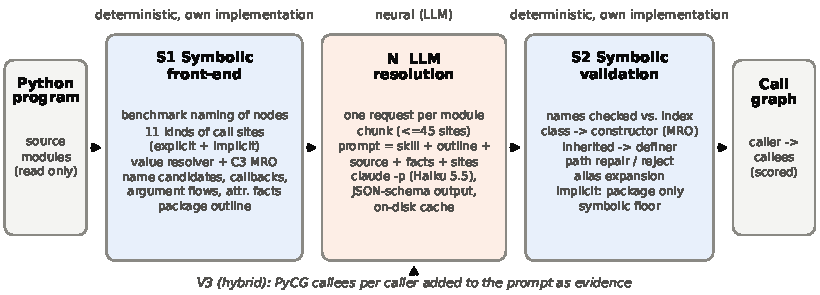
\includegraphics[width=0.92\textwidth]{figures/pipeline.pdf}
  \caption{Architecture of NSCG. S1 and S2 are symbolic and deterministic; N is
  the only neural stage. The hybrid variant V3 additionally shows PyCG's
  callees to the LLM.}
  \label{fig:pipeline}
\end{figure*}

\subsection{S1: symbolic front-end}
\label{sec:s1}

The front-end parses every module with Python's \texttt{ast} module (code is
never imported or run) and computes:

\textbf{Nodes with benchmark names.} Modules, functions, methods and lambdas
get the dotted names of the conventions; a lambda is numbered by the source
position of its \texttt{lambda} keyword among the lambdas of the scope that
evaluates it, and class bodies and comprehensions are transparent for the
caller attribution. On the four packages our node sets equal the ground-truth
node sets exactly (634 nodes); on the micro-benchmark they are equal in 613 of
622 cases (the others contain modules that never run).

\textbf{Call sites.} A walker attributes each site to the node whose execution
makes it (a decorator or default value to the enclosing scope, a class body to
the function or module that runs it). It finds 13 kinds of sites: explicit
calls, decorators, \texttt{raise C} without a call, and class creation
(\texttt{\_\_init\_subclass\_\_}, metaclass hooks, \texttt{\_\_set\_name\_\_}),
plus nine implicit kinds: \texttt{with}, iteration (\texttt{for},
comprehensions, \texttt{yield from}, unpacking), \texttt{**} mappings,
\texttt{await}, operators (binary, augmented, unary, comparisons and
\texttt{in}), subscripts (get/set/del), property accesses, truth tests and
f-string formatting. An implicit site is kept only if some package function has
a matching special-method name, because only package callees of implicit calls
are edges. The four packages yield 1,973 sites (the ground-truth ledgers have
1,846 sites of the kinds that need an entry).

\textbf{Symbolic pre-resolution.} A flow-insensitive, demand-driven resolver
maps an expression to abstract values: package functions, bound methods,
decorated definitions, classes, instances, modules, \texttt{super()} objects,
parameters, and outside paths/instances. Names are looked up through Python's
scoping rules (local, enclosing, \texttt{global}/\texttt{nonlocal}, module,
builtins), imports including relative and star imports, assignments (followed
recursively up to depth~6), the C3 MRO of package classes (an outside base
terminates the lookup and names the member through that base), instance
attributes through \emph{attribute facts} (\texttt{self.x = e} in any class of
the receiver's hierarchy), and return expressions of called functions. A call of
a class targets what instantiation runs (first \texttt{\_\_init\_\_} of the MRO,
inside or named through the nearest outside base, a package
\texttt{\_\_new\_\_}, a metaclass \texttt{\_\_call\_\_}). A resolution is
marked \emph{certain} when the callee is a static path with one binding (a
plain name bound once, or an attribute chain on a module).

\textbf{Candidates and facts.} The resolver is deliberately cheap, so it misses
values. To give the LLM a complete menu, every site also gets (i) the package
functions whose name equals the called name, the constructors of package
classes with that name, and the overriding methods of the receiver class's
package subclasses (receivers can be subclass instances); (ii) the package
functions and classes passed as arguments (callbacks); (iii) for a call of a
parameter, the package functions that resolved package calls pass for that
parameter (one level of argument flow); (iv) the attribute assignments that
matter for the chunk's attribute calls; and (v) a symbolic outline of the
whole package (imports, functions with parameters and decorators, classes with
bases, MRO, methods, properties and class attributes) used for naming callees
in other modules. \emph{V2.1 only:} at a call of a library method on a package
instance whose class derives from that library, (vi) the methods of the
package's subclasses of that library's classes, which the library may call back
(template methods, hooks).

\subsection{N: LLM resolution of call sites}

The sites of a module are split into chunks of at most 45, and each chunk
becomes one request. The prompt contains: a fixed ``skill'' that restates the
call-graph semantics in 40 lines (node names, which implicit calls and
callbacks are edges, the MRO rule for constructors, how outside callees are
named); instructions on how to treat the symbolic information (pre-resolutions
are usually right when certain, name candidates are naive and must be filtered
by types and hierarchy, implicit sites admit only package callees, never invent
a package name); the outline and the attribute facts; the numbered source of
the module (or, for modules above 700 lines, the window that holds the chunk's
callers plus the import header); and one line per site with its id, caller,
position, kind, text and symbolic information. The model answers a JSON object
\texttt{\{"sites": [\{"id", "callees"\}]\}}, enforced by a JSON schema.

We run the model through headless Claude Code (\texttt{claude -p}) with all
tools disabled, no settings, no project memory and an empty working directory,
so each request is a pure, stateless LLM call; Claude Code here is only the
transport and the structured-output enforcement. The default model is Claude
Haiku~5.5 (the cheapest current Claude model); we also report Claude
Sonnet~5.5. Every request and answer is stored in a content-addressed cache,
so all reported numbers can be replayed offline, and its token usage and cost
are recorded.

\subsection{S2: symbolic validation}

The model's names are checked against the definition index of S1. A name that
is a package node is kept; a package class is replaced by what instantiating it
runs; \texttt{pkg.C.m} for a method that \texttt{C} inherits is mapped through
the MRO to the defining class; a package-looking name that names nothing is
repaired if exactly one node shares its last two components (a wrong module
path) and is otherwise rejected as a hallucination; an outside name whose head
is a local import alias is expanded; at implicit sites outside names are
dropped; and, as a \emph{symbolic floor}, certain resolutions of S1 are always
kept. If the model omits a site, its symbolic resolution is used. Every
decision is counted (Table~\ref{tab:validation}).

\subsection{Variants and design iterations}
\label{sec:variants}

To find out which components matter, we built the design incrementally and
kept each version as a variant that runs on the same subjects:

\begin{itemize}[leftmargin=*]
\item \textbf{S1-only} (\texttt{nscg-sym}): the symbolic pre-resolutions alone,
no LLM --- the symbolic half of NSCG as an analysis of its own.
\item \textbf{V0, LLM-only}: the model receives the skill, the outline and the
source and writes the call graph \texttt{\{caller: [callees]\}} directly. This
is the obvious way to use an LLM and our neural reference point.
\item \textbf{V1, sites without hints}: S1 enumerates the sites, but the prompt
contains no per-site symbolic information and no facts; S2 validates.
\item \textbf{V2, NSCG}: the full design of Sections~\ref{sec:s1}--S2.
\item \textbf{V2.1}: the revision after the error analysis of V2
(Section~\ref{sec:rq3}): library-hook candidates (vi) and three fixes of the
validator's alias expansion that wrongly rewrote correct names
(\texttt{time.time}$\rightarrow$\texttt{time.time.time} after \texttt{from time
import time}, \texttt{invoke.Argument}$\rightarrow$\texttt{invoke.\_\_version\_\_.Argument}
after \texttt{from invoke import \_\_version\_\_ as invoke}, and
\texttt{builtins.all} instead of \texttt{<builtin>.all}).
\item \textbf{V3, hybrid}: V2/V2.1 plus, for each caller of the chunk, the
callees that PyCG-2026 reports, presented as evidence that can be wrong.
We also evaluate the offline set combinations PyCG\,$\cup$\,NSCG and
PyCG\,$\cap$\,NSCG.
\end{itemize}

\subsection{What is original, and relation to prior work}

All of S1, S2, the prompts, the skill text, the variants and the evaluation
scripts were written for this project. We reuse only infrastructure: the
benchmark, its ground truths, its runner and scorer (so that every tool is
scored identically), PyCG itself as the baseline and as the evidence source of
V3, and Claude Code as the LLM transport. The design is related to, but
differs from, prior neuro-symbolic work. Learned call-graph pruning
(CGPruner~\cite{utture2022cgpruner}, AutoPruner~\cite{le2022autopruner})
removes edges from a sound static graph with a classifier; NSCG instead lets
the LLM choose among symbolic candidates and add callees, and its symbolic
stages constrain the LLM rather than the other way round. LLM-based data-flow
analysis such as LLMDFA~\cite{wang2024llmdfa} and LLM-assisted static bug
detection such as LLift~\cite{li2024llift} and IRIS~\cite{li2025iris} use the
LLM for sources, sinks, summaries or path feasibility of a different analysis
task; NSCG uses it for value resolution at call sites and constrains it with a
generated candidate menu and a symbolic validator. Studies that ask LLMs for
Python call graphs on micro-benchmarks~\cite{venkatesh2024emergence} evaluate
our V0 setting; we compare it with our neuro-symbolic design on real packages.

\section{Evaluation}
\label{sec:eval}

\subsection{Evaluation setting}
\label{sec:setup}

\textbf{Research questions.}
\textbf{RQ1} How accurate is \nscg compared with PyCG-2021 and PyCG-2026?
\textbf{RQ2} What does each component of \nscg contribute, and how much does the
model matter?
\textbf{RQ3} Which edges does each approach get wrong, and why?
\textbf{RQ4} Do the LLM's answers depend on memorised names, and are they stable
across runs?
\textbf{RQ5} Do hybrids of PyCG and \nscg combine their strengths?

\textbf{Subjects.} We use the two benchmarks of the PyCG evaluation repository~\cite{pycgeval2026}
(commit \texttt{8a2e52c}), because they are the only Python call-graph
benchmarks with executable baselines and carefully defined ground truths.
(i) The \emph{micro-benchmark}: the 622 cases up to Python~3.12 (the cohort the
evaluation uses to compare tools), small programs of 34 feature categories
(classes, decorators, dynamic features, imports, standard library, \dots), each
with a ground truth validated against a dynamic trace. (ii) Four packages of the
\emph{macro-benchmark} (Table~\ref{tab:subjects}), whose ground truths are
call-site ledgers written by hand, checked against the traces of the packages'
test suites, and audited four times. Given a limited budget and the course's
guidance of three to four real projects, we selected them to cover both regimes
of the baseline: two where PyCG-2026 is strong (autojump, a small script-like
utility; jmespath, an interpreter with visitor dispatch through
\texttt{getattr}) and two where it is weak (fabric, which subclasses and is
called back by the Invoke framework; funcy, a higher-order functional library),
two from the ICSE~2021 set and two from later batches.

\begin{table}[t]
  \caption{The four packages (sources at the pinned commits of the benchmark).
  Edges in/out: ground-truth edges inside / outside the package. Sites: call
  sites found by the \nscg front-end.}
  \label{tab:subjects}
  \small
  \setlength{\tabcolsep}{3.2pt}
  \begin{tabular}{l l r r r r r r}
\toprule
Package & batch & LOC & mod. & nodes & edges in/out & sites & PyCG F1\\
\midrule
autojump & ICSE'21 & 488 & 3 & 46 & 35/100 & 139 & 0.95 \\
fabric & ICSE'21 & 2,303 & 12 & 93 & 99/252 & 377 & 0.71 \\
jmespath & 1 & 1,675 & 8 & 190 & 310/120 & 470 & 0.99 \\
funcy & 5 & 2,392 & 16 & 305 & 511/475 & 987 & 0.65 \\
\bottomrule
\end{tabular}

\end{table}

\textbf{Criteria.} Edge precision, recall and $F_1$, computed by the official
scorer (\texttt{evaluation/common/score.py}, raw names) separately for callees
inside the package (the headline, as in the PyCG evaluation) and outside it; for
the micro-benchmark also the number of cases whose graph equals the ground truth
exactly. A run that fails counts every edge of its program as missed.

\textbf{Setup.} All runs use one machine (Ubuntu 22.04, 128 cores, 755\,GB
RAM) and Python~3.14.3. The baselines run through the official runner with a
30-minute and 16\,GiB limit per program (PyCG-2021 timed out on funcy, as in
the PyCG evaluation). \nscg uses Claude Haiku~5.5 (and Sonnet~5.5 for RQ2)
through \texttt{claude -p} 2.1.321, 16 requests in parallel, default sampling
(the CLI exposes no temperature), one sample per request; RQ4 repeats the
macro runs with independent samples. The same subjects, entry points and
package roots are given to every tool, and no tool sees the ground truth. The
skill text of the prompts was written from the benchmark's documented
conventions (the same information the PyCG authors had), and the prompts were
developed on a handful of micro cases only; the four packages were not used to
tune the prompts before the V2 run. The total LLM cost of every request of the
study is US\$21.15 (Table~\ref{tab:cost}), of which the
Sonnet runs are three quarters. Money was not the binding constraint; the time
frame of the project (one week of wall-clock time, including the 30-minute
limits of the baselines) and the course's guidance limited the macro
evaluation to four packages, and we chose the cheapest model as the default so
that every variant could be run on all subjects.


\begin{table*}[t]
  \caption{Accuracy of every tool (official scorer, raw names). Inside: edges
  whose callee is in the analysed package (the headline); outside: edges to
  builtins, the standard library and other packages; exact: micro cases whose
  graph equals the ground truth. Bold: best single tool in a column. All \nscg
  variants use Haiku~5.5; Sonnet rows are discussed in RQ2. PyCG-2021 timed out
  on funcy (all its edges count as missed).}
  \label{tab:main}
  \small
  \setlength{\tabcolsep}{3.6pt}
  \begin{tabular}{l rrr rr r rrr rrr}
\toprule
& \multicolumn{6}{c}{Micro-benchmark (622 cases)} & \multicolumn{6}{c}{Four packages (1,973 sites)}\\
\cmidrule(lr){2-7}\cmidrule(lr){8-13}
& \multicolumn{3}{c}{inside} & \multicolumn{2}{c}{outside} & & \multicolumn{3}{c}{inside} & \multicolumn{3}{c}{outside}\\
\cmidrule(lr){2-4}\cmidrule(lr){5-6}\cmidrule(lr){8-10}\cmidrule(lr){11-13}
Tool & P & R & F1 & P & R & exact & P & R & F1 & P & R & F1\\
\midrule
PyCG-2021 (baseline) & 0.868 & 0.605 & 0.713 & 0.862 & 0.660 & 201 & 0.927 & 0.308 & 0.462 & 0.869 & 0.288 & 0.432 \\
PyCG-2026 (baseline) & 0.925 & 0.936 & 0.931 & \textbf{0.996} & 0.962 & \textbf{466} & 0.894 & 0.712 & 0.793 & 0.879 & 0.827 & 0.852 \\
\midrule
S1 only (no LLM) & 0.891 & 0.606 & 0.721 & 0.906 & 0.850 & 118 & 0.963 & 0.550 & 0.700 & 0.891 & 0.714 & 0.792 \\
V0 LLM-only & 0.893 & \textbf{0.995} & \textbf{0.941} & 0.956 & 0.829 & 265 & 0.958 & 0.685 & 0.799 & 0.965 & 0.764 & 0.853 \\
V1 sites, no hints & 0.903 & 0.969 & 0.935 & 0.938 & 0.949 & 258 & 0.967 & 0.703 & 0.814 & 0.915 & 0.826 & 0.868 \\
V2 NSCG & 0.892 & 0.974 & 0.932 & 0.931 & 0.939 & 251 & 0.912 & 0.730 & 0.811 & 0.880 & 0.846 & 0.863 \\
V2.1 NSCG (final) & 0.889 & 0.974 & 0.930 & 0.929 & 0.939 & 251 & 0.913 & 0.732 & 0.812 & 0.899 & 0.859 & 0.879 \\
V3 hybrid (V2+PyCG) & -- & -- & -- & -- & -- & -- & 0.923 & 0.729 & 0.815 & 0.898 & 0.864 & 0.880 \\
V3 hybrid (V2.1+PyCG) & -- & -- & -- & -- & -- & -- & 0.923 & 0.729 & 0.815 & 0.917 & 0.874 & \textbf{0.895} \\
\midrule
PyCG-2026 $\cup$ V2.1 & 0.875 & 0.994 & 0.931 & 0.932 & 0.989 & 428 & 0.844 & 0.746 & 0.792 & 0.831 & 0.902 & 0.865 \\
PyCG-2026 $\cap$ V2.1 & 0.943 & 0.916 & 0.929 & 0.995 & 0.911 & 450 & 0.977 & 0.698 & 0.814 & 0.967 & 0.784 & 0.866 \\
\midrule
V0 LLM-only, Sonnet & -- & -- & -- & -- & -- & -- & 0.944 & 0.619 & 0.748 & 0.974 & 0.753 & 0.849 \\
V2.1 NSCG, Sonnet & 0.912 & 0.973 & 0.941 & 0.930 & 0.926 & 273 & 0.928 & 0.739 & 0.823 & 0.950 & 0.822 & 0.882 \\
\bottomrule
\end{tabular}

\end{table*}

\subsection{RQ1: accuracy against the symbolic baselines}
\label{sec:rq1}

Table~\ref{tab:main} and Figure~\ref{fig:pr} give the aggregate results, and
Table~\ref{tab:projects} the results per package.

\textbf{Four packages.} The final design V2.1 reaches inside
P\,\R{macro-ins-p-nscg-v21} / R\,\R{macro-ins-r-nscg-v21} /
$F_1$\,\R{macro-ins-f1-nscg-v21}, against \R{macro-ins-p-pycg-2026} /
\R{macro-ins-r-pycg-2026} / \R{macro-ins-f1-pycg-2026} for PyCG-2026: slightly
higher precision and recall in aggregate, but not uniformly, and the
aggregate gap ($+$0.019 $F_1$) is only about twice the run-to-run standard deviation of
\nscg (RQ4), so we read it as parity. \nscg is better on autojump
(PyCG-2026 reports four lambdas that the functions only hand to lazy
\texttt{map}/\texttt{filter} objects returned to the caller, which the
callback rule attributes to the caller; \nscg gets all 35 edges right) and on
funcy, slightly better on jmespath, and on fabric it trades precision
(\R{fabric-in-p-nscg-v21} vs.\ \R{fabric-in-p-pycg-2026}) for recall
(\R{fabric-in-r-nscg-v21} vs.\ \R{fabric-in-r-pycg-2026}). PyCG-2021 is far
behind (inside $F_1$ \R{macro-ins-f1-pycg-2021}): it misses most edges through
library values and timed out on funcy (even without funcy its recall on the other
three packages is clearly lower, Table~\ref{tab:projects}). On outside edges \nscg also leads
($F_1$ \R{macro-out-f1-nscg-v21} vs.\ \R{macro-out-f1-pycg-2026}).

\textbf{Micro-benchmark.} The picture is different. Every LLM-based variant has
a much higher inside recall than PyCG-2026 (V2.1 \R{micro-ins-r-nscg-v21}, V0
\R{micro-ins-r-llm-only} vs.\ \R{micro-ins-r-pycg-2026}) but a lower precision
(\R{micro-ins-p-nscg-v21} vs.\ \R{micro-ins-p-pycg-2026}), so the inside $F_1$
values are close, while PyCG-2026 is clearly better on outside names
(P\,\R{micro-out-p-pycg-2026} vs.\ \R{micro-out-p-nscg-v21}) and produces the
exact graph for \R{micro-exact-pycg-2026} of 622 cases against
\R{micro-exact-nscg-v21} for V2.1. The LLM variants are \emph{less exact but
more complete}: they rarely miss a call, but they add plausible edges that the
precise semantics excludes and spell outside callees differently.
Figure~\ref{fig:categories} shows where the tools differ most. The LLM-based
variants win on \emph{dynamic} features (\texttt{eval} of a constructed string,
\texttt{getattr}/\code{operator.methodcaller}, \code{sys.modules}, monkey
patching), on the standard library, on context managers and on missing external
modules --- cases where reading the code as a developer does beats an
abstraction; PyCG-2026 wins on exactly specified semantics: tuples, strings,
\texttt{match}, argument binding, async code and class hierarchies.

\begin{figure*}[t]
  \centering
  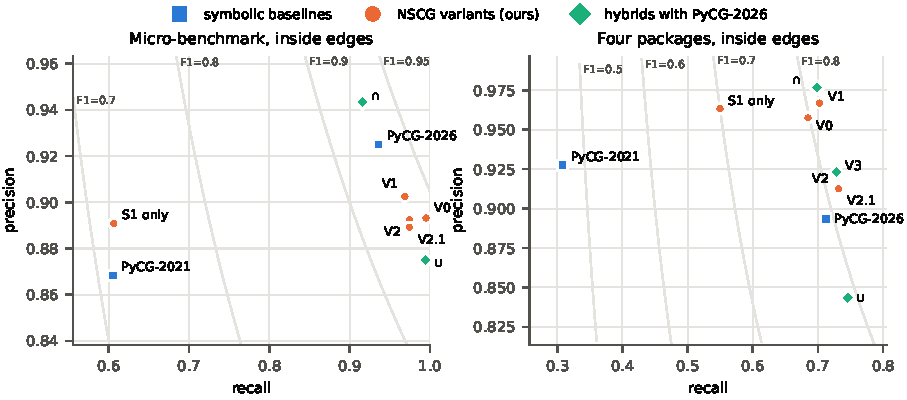
\includegraphics[width=0.86\textwidth]{figures/pr.pdf}
  \caption{Precision and recall of inside edges; grey lines are $F_1$
  iso-curves. Left: micro-benchmark; right: the four packages (PyCG-2021 timed
  out on funcy, whose edges count as missed).}
  \label{fig:pr}
\end{figure*}

\begin{table*}[t]
  \caption{Inside edges per package (P / R / $F_1$). PyCG-2021 timed out on funcy.}
  \label{tab:projects}
  \small
  \setlength{\tabcolsep}{3.4pt}
  \begin{tabular}{l rrr rrr rrr rrr }
\toprule
& \multicolumn{3}{c}{autojump} & \multicolumn{3}{c}{fabric} & \multicolumn{3}{c}{jmespath} & \multicolumn{3}{c}{funcy}\\
\cmidrule(lr){2-4}\cmidrule(lr){5-7}\cmidrule(lr){8-10}\cmidrule(lr){11-13}
& P & R & F1 & P & R & F1 & P & R & F1 & P & R & F1\\
\midrule
PyCG-2021 & 1.00 & 0.89 & 0.94 & 0.92 & 0.46 & 0.62 & 0.92 & 0.70 & 0.79 & \multicolumn{3}{c}{timeout} \\
PyCG-2026 & 0.90 & 1.00 & 0.95 & 0.96 & 0.56 & 0.71 & 0.97 & 1.00 & 0.99 & 0.81 & 0.55 & 0.65 \\
S1 only & 1.00 & 0.89 & 0.94 & 0.96 & 0.47 & 0.64 & 1.00 & 0.72 & 0.83 & 0.93 & 0.44 & 0.60 \\
V0 & 1.00 & 1.00 & 1.00 & 0.84 & 0.62 & 0.71 & 1.00 & 1.00 & 1.00 & 0.94 & 0.49 & 0.64 \\
V2 & 1.00 & 1.00 & 1.00 & 0.88 & 0.62 & 0.73 & 1.00 & 0.99 & 1.00 & 0.83 & 0.57 & 0.68 \\
V2.1 & 1.00 & 1.00 & 1.00 & 0.89 & 0.64 & 0.74 & 1.00 & 0.99 & 1.00 & 0.83 & 0.57 & 0.68 \\
V3 (V2.1) & 1.00 & 0.89 & 0.94 & 0.89 & 0.64 & 0.74 & 1.00 & 1.00 & 1.00 & 0.86 & 0.57 & 0.69 \\
$\cup$ & 0.90 & 1.00 & 0.95 & 0.89 & 0.64 & 0.74 & 0.97 & 1.00 & 0.99 & 0.73 & 0.60 & 0.66 \\
\bottomrule
\end{tabular}

\end{table*}

\begin{figure}[t]
  \centering
  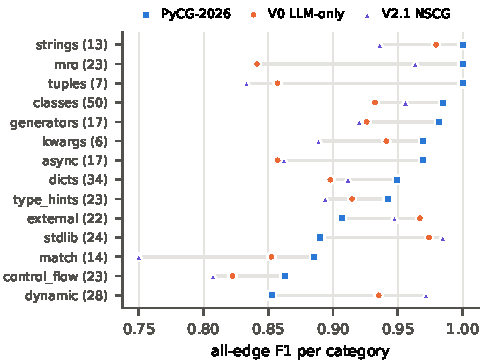
\includegraphics[width=0.95\columnwidth]{figures/categories.pdf}
  \caption{All-edge $F_1$ per micro category (number of cases in parentheses)
  for the 14 categories where PyCG-2026, V0 and V2.1 differ most.}
  \label{fig:categories}
\end{figure}

\subsection{RQ2: what each component contributes}
\label{sec:rq2}

\textbf{The symbolic front-end alone} (S1 only) is precise but incomplete:
inside P\,\R{macro-ins-p-nscg-sym} but R\,\R{macro-ins-r-nscg-sym} on the
packages, recall \R{micro-ins-r-nscg-sym} on micro. Its resolver is deliberately
cheap; it is not meant to be an analysis of its own, yet it already matches
PyCG-2021's micro accuracy (all-edge $F_1$ \R{micro-all-f1-nscg-sym} vs.\
\R{micro-all-f1-pycg-2021}).

\textbf{The LLM alone} (V0) is a strong baseline --- one of the main surprises
of the study. On the packages it has higher precision than V2.1
(\R{macro-ins-p-llm-only}) but lower recall (\R{macro-ins-r-llm-only}); on
micro it has the best inside recall of all single tools. Its weaknesses are
systematic rather than random: it omits calls that are easy to overlook in a
whole-program answer (V0 loses most of its micro \emph{mro} points by omitting the
\code{<builtin>.super} edge that every \texttt{super()} call creates, which
\nscg's site enumeration never misses), it names outside callees less
consistently, and it cannot be checked.

\textbf{Per-site hints} (V1$\rightarrow$V2) are a double-edged sword. With the
same sites but no symbolic information, V1 is the most \emph{precise}
LLM variant on the packages (P\,\R{macro-ins-p-nscg-nohints}, R\,\R{macro-ins-r-nscg-nohints});
adding resolutions, name candidates, callbacks and facts raises recall to
\R{macro-ins-r-nscg} but lowers precision to \R{macro-ins-p-nscg}, so $F_1$ is
unchanged (\R{macro-ins-f1-nscg-nohints} vs.\ \R{macro-ins-f1-nscg}). The model
tends to \emph{accept} plausible candidates: 57 of V2's inside false
positives were proposed by the front-end (Table~\ref{tab:errors}), most of them
name matches in funcy (e.g.\ every \code{__getitem__} of the package at a
subscript of an unknown mapping).

\textbf{The validator} turned out to be nearly neutral (a negative result).
Given the outline and the candidates, the model rarely invents package names:
on the packages it added only \R{err-fp-llm-added-nscg-v21} wrong package
callees that no component proposed, and the validator rejected a single unknown
package name in V2.1 (Table~\ref{tab:validation}). Without any validation (raw
names), V2.1 scores inside $F_1$ \R{macro-ins-f1-nscg-v21-novalidate} and
outside $F_1$ \R{macro-out-f1-nscg-v21-novalidate}, i.e.\ the same as with it.
V2's alias expansion was in fact \emph{harmful} (outside $F_1$
\R{macro-out-f1-nscg}); the three fixes of V2.1 only removed that harm. The
symbolic floor is slightly harmful on micro (exact cases
\R{micro-exact-nscg-v21} with it, \R{micro-exact-nscg-v21-nofloor} without;
Section~\ref{sec:discussion}).

\textbf{Library hooks and the model.} With Haiku, the library hooks of V2.1
recovered only two Fabric edges: at \texttt{self.\_run(runner, command)} in
\code{Connection.run}, the prompt listed the methods of Fabric's
\texttt{Remote} runner that Invoke's \code{Runner.run} calls back, but Haiku
kept only \code{invoke.Context._run}. With Sonnet~5.5 and the same prompt,
the model used its knowledge of Invoke and recovered 18 of these callbacks
(\code{Connection.run}/\texttt{sudo} $\rightarrow$ \code{Remote.start},
\code{read_proc_stdout}, \code{send_interrupt}, \dots), raising Fabric's
recall from \R{fabric-in-r-nscg-v21} to \R{fabric-in-r-nscg-v21@sonnet}. Overall,
Sonnet improves V2.1 moderately (inside $F_1$ \R{macro-ins-f1-nscg-v21@sonnet}
on the packages, \R{micro-ins-f1-nscg-v21@sonnet} on micro) at about ten times
the cost. As an LLM-only analyzer, however, Sonnet is \emph{worse} than Haiku
(\R{macro-ins-f1-llm-only@sonnet} vs.\ \R{macro-ins-f1-llm-only}), mainly through
lower recall (jmespath \R{jmespath-in-r-llm-only@sonnet}): the structure that
\nscg imposes matters more than the model.

\begin{table}[t]
  \caption{Decisions of the validator S2 (callee names over all sites): package / outside names kept,
  unknown package names rejected, \texttt{C.\_\_init\_\_} mapped to the constructor through the MRO,
  and certain symbolic resolutions added by the floor. The other rules (path repair, class$\to$constructor,
  inherited$\to$definer, outside names at implicit sites, and V2.1's \texttt{builtins.X} renaming) never fired.}
  \label{tab:validation}
  \small
  \setlength{\tabcolsep}{4pt}
  \begin{tabular}{l l rrrrr}
\toprule
Run & bench. & kept in & kept out & rejected & init$\to$ctor & floor\\
\midrule
V2 & micro & 1438 & 490 & 5 & 2 & 18 \\
V2 & macro & 928 & 1093 & 3 & 0 & 16 \\
V2.1 & micro & 1444 & 493 & 5 & 2 & 16 \\
V2.1 & macro & 930 & 1095 & 1 & 0 & 5 \\
V1 & micro & 1405 & 489 & 1 & 0 & 28 \\
V1 & macro & 843 & 1034 & 12 & 0 & 16 \\
\bottomrule
\end{tabular}

\end{table}


\subsection{RQ3: successes and failures}
\label{sec:rq3}

Table~\ref{tab:errors} labels every false negative and false positive on the
four packages. The labels use what the front-end proposed at the sites of the
caller.

\begin{table*}[t]
  \caption{Error taxonomy on the four packages. FN inside: \emph{no hint} -- no
  site of the caller proposed the callee; \emph{dropped} -- proposed but
  dropped by the LLM. FN outside: \emph{misnamed} -- the tool has an outside
  callee of the same caller with the same last name component. FP inside:
  \emph{from hint} -- proposed by the front-end and kept; \emph{added} -- added
  by the LLM. FP outside: \emph{misnamed} -- the ground truth has a callee with
  the same last component.}
  \label{tab:errors}
  \small
  \begin{tabular}{l rrrr rrrr}
\toprule
& \multicolumn{4}{c}{false negatives} & \multicolumn{4}{c}{false positives}\\
\cmidrule(lr){2-5}\cmidrule(lr){6-9}
& \multicolumn{2}{c}{inside} & \multicolumn{2}{c}{outside} & \multicolumn{2}{c}{inside} & \multicolumn{2}{c}{outside}\\
Tool & no hint & dropped & misnamed & omitted & from hint & added & misnamed & spurious\\
\midrule
S1 only & 389 & 41 & 56 & 215 & 20 & 0 & 63 & 20 \\
V0 & 276 & 25 & 24 & 199 & 16 & 13 & 10 & 16 \\
V2 & 255 & 3 & 64 & 82 & 57 & 10 & 61 & 48 \\
V2.1 & 253 & 3 & 53 & 80 & 57 & 10 & 43 & 48 \\
V3 (V2.1) & 253 & 6 & 53 & 66 & 53 & 5 & 41 & 34 \\
\bottomrule
\end{tabular}

\end{table*}

\textbf{The LLM filters; it rarely discovers.} \R{err-fn-no-evidence-nscg-v21}
of V2.1's \R{macro-ins-fn-nscg-v21} missed inside edges had no hint at any site
of the caller, and only \R{err-fp-llm-added-nscg-v21} inside false positives
were added by the model without a hint. The hints decide what \nscg can find;
the three repetitions of RQ4 have \emph{identical} inside recall. Where the hint
is there, the model is good at keeping the right callees: only
\R{err-fn-rejected-nscg-v21} proposed true edges were dropped.

\textbf{A hard core that no tool finds.} Of V2.1's
\R{macro-ins-fn-nscg-v21} missed inside edges, 243 are also missed by
PyCG-2026 (which misses only 32 inside edges that V2.1 finds). They come from
two mechanisms. (1) \emph{Library callbacks}: Fabric's \code{Connection.run}
hands a \texttt{Remote} runner to Invoke, whose \code{Runner.run} calls back
\texttt{start}, \code{read_proc_stdout}, \code{send_start_message} and
others; the ground truth reads Invoke's code to find them, PyCG-2026 does not
model outside code that calls back, and \nscg's model did not supply the
knowledge. (2) \emph{Documented roles}: funcy's ground truth gives a parameter
such as \texttt{pred} of \code{_lfilter} every package function that the
documentation or the tests pass in that role (\texttt{isnone}, \texttt{even},
the lambdas made by \code{re_tester}, \dots); no tool reads the
documentation, so most of funcy's \R{funcy-in-fn-nscg-v21} missed edges are
of this kind.

\textbf{Where reading beats abstracting.} In jmespath, the metaclass
\code{FunctionRegistry} registers only the methods whose name starts with
\code{_func_}, and \code{call_function} calls the registered function.
PyCG-2026 cannot evaluate the string filter and reports every method of the
class (7 false positives such as \code{_type_check}); \nscg calls only the
\code{_func_} methods. In the micro-benchmark, \nscg resolves
\texttt{eval(measure + "()")} with \texttt{measure = "area"} to
\code{main.area}, and similar string-built dispatches, which PyCG treats as
unknowable by design.

\textbf{Where abstracting beats reading.} PyCG-2026's 466 exact micro graphs
come from strictly applied conventions: it never adds an edge that the
semantics excludes, names every outside callee through typeshed, and handles
argument binding and \texttt{match} precisely. \nscg's micro false positives
are mostly over-approximations accepted from the flow-insensitive hints (a dict
entry overwritten before the call; a lazily built \texttt{map} that is never
consumed) and \emph{misnamed outside callees} (\code{<builtin>.iter.__next__}
for \code{builtins.list_iterator.__next__},
\code{paramiko.transport.Transport.open_session} for the benchmark's access
path \code{paramiko.client.SSHClient.get_transport.open_session}). Of
V2.1's 224 outside errors on the packages, 96 (43\%) are such near misses with
the right last name component (Table~\ref{tab:errors}).

\textbf{Unexpected behaviours.} (i) Evidence can \emph{hurt}: in the hybrid
V3, the model dropped four lambda callbacks of \texttt{autojump} (three in
\code{autojump_data.load}) that both PyCG-2026 and V2 had found and that
PyCG's evidence listed. (ii) The validator itself had bugs that only
the error analysis exposed (the three alias expansions of V2.1). (iii) V0 is
more precise than V2 on the packages, the opposite of what we designed for.

\subsection{RQ4: memorisation and stability}
\label{sec:rq4}

\textbf{Renaming probe.} Both benchmarks are public on GitHub, so the LLM may
have seen the programs, and even the micro-benchmark's ground-truth files. To
test whether its accuracy depends on familiar names, we consistently renamed
every package-defined function and class of the micro cases (to names like
\code{q3f1_0}) where this is syntactically safe, rewrote the ground truth,
and kept the 580 cases whose renamed ground truth the benchmark's own dynamic
validator still accepts. Table~\ref{tab:probe} compares the same 580 cases
before and after renaming.

\begin{table}[t]
  \caption{Renaming probe on 580 micro cases (inside edges; all-edge $F_1$;
  exact cases). Symbolic tools are name-invariant by construction.}
  \label{tab:probe}
  \setlength{\tabcolsep}{3pt}
  \resizebox{\columnwidth}{!}{\begin{tabular}{l rrr rrr rr rr}
\toprule
& \multicolumn{3}{c}{original, inside} & \multicolumn{3}{c}{renamed, inside} & \multicolumn{2}{c}{all-edge F1} & \multicolumn{2}{c}{exact}\\
\cmidrule(lr){2-4}\cmidrule(lr){5-7}\cmidrule(lr){8-9}\cmidrule(lr){10-11}
Tool & P & R & F1 & P & R & F1 & orig. & ren. & orig. & ren.\\
\midrule
PyCG-2026 & 0.924 & 0.946 & 0.935 & 0.924 & 0.946 & 0.935 & 0.946 & 0.946 & 441 & 441 \\
PyCG-2021 & 0.868 & 0.613 & 0.719 & 0.868 & 0.613 & 0.719 & 0.724 & 0.724 & 185 & 185 \\
S1 only & 0.889 & 0.613 & 0.725 & 0.889 & 0.613 & 0.725 & 0.767 & 0.767 & 114 & 114 \\
V0 LLM-only & 0.893 & 0.996 & 0.942 & 0.902 & 0.998 & 0.948 & 0.925 & 0.927 & 261 & 264 \\
V2.1 NSCG & 0.888 & 0.976 & 0.930 & 0.893 & 0.976 & 0.933 & 0.928 & 0.932 & 247 & 255 \\
\bottomrule
\end{tabular}
}
\end{table}

Renaming does not hurt the LLM-based analyzers: V0 goes from inside $F_1$
\R{probe-orig-f1-llm-only} to \R{probe-ren-f1-llm-only} and V2.1 from
\R{probe-orig-f1-nscg-v21} to \R{probe-ren-f1-nscg-v21}, with as many or more
exact cases (V2.1: \R{probe-orig-exact-nscg-v21} $\rightarrow$
\R{probe-ren-exact-nscg-v21}), and the symbolic tools are unchanged, as they
must be. The micro-benchmark results therefore do not depend on recognising
the original identifiers or on recalling the published \code{callgraph.json}
files, whose names no longer match. The probe cannot exclude that the model has
learned the benchmark's \emph{structure} (the cases are small idioms that also
occur everywhere else), and it does not cover the packages, which are too large
to rename safely; we discuss this in Section~\ref{sec:threats}.


\textbf{Stability.} Three independent runs of V2.1 on the packages
(Table~\ref{tab:repeats}) have a standard deviation of \R{repeat-sd-f1} in
inside $F_1$; \R{repeat-agree} edges reported by any run are reported by all
three (\R{repeat-agree-pct}\%). All variation is in precision
(\R{repeat-min-p}--\R{repeat-max-p}, mostly funcy's name-matched
\code{__getitem__} candidates); recall is the same in every run. The differences between the variants in RQ2 that
are smaller than about two standard deviations should therefore not be read
as real effects.

\begin{table}[t]
  \caption{Three runs of V2.1 (Haiku) on the four packages.}
  \label{tab:repeats}
  \small
  \begin{tabular}{l rrr rr}
\toprule
Metric (4 packages) & run 1 & run 2 & run 3 & mean & s.d.\\
\midrule
inside P & 0.913 & 0.890 & 0.936 & 0.913 & 0.023 \\
inside R & 0.732 & 0.732 & 0.732 & 0.732 & 0.000 \\
inside F1 & 0.812 & 0.803 & 0.821 & 0.812 & 0.009 \\
outside P & 0.899 & 0.908 & 0.908 & 0.905 & 0.005 \\
outside R & 0.859 & 0.845 & 0.847 & 0.850 & 0.008 \\
outside F1 & 0.879 & 0.875 & 0.876 & 0.877 & 0.002 \\
\bottomrule
\end{tabular}

\end{table}

\subsection{RQ5: hybrids}
\label{sec:rq5}

The two kinds of analyzers make different false positives (of V2.1's 67 and
PyCG-2026's 81 inside false positives on the packages only 16 are shared) but
largely the same false negatives, so combinations raise precision more easily
than recall. The edge \emph{union} has the highest inside recall on the packages
(\R{macro-ins-r-union--pycg-2026--nscg-v21}) and nearly the highest on micro
(\R{micro-ins-r-union--pycg-2026--nscg-v21}) at a loss of precision; the \emph{intersection} is the most precise configuration
(\R{macro-ins-p-inter--pycg-2026--nscg-v21} / \R{micro-ins-p-inter--pycg-2026--nscg-v21})
and has the best micro inside precision of all. Giving PyCG's callees to the LLM
(V3) yields the best outside $F_1$ (\R{macro-out-f1-nscg-hybrid-v21}) and a
small inside gain (\R{macro-ins-f1-nscg-hybrid-v21}): the model uses PyCG's
typeshed-based outside names, but it does not simply copy PyCG, and the inside
edges that both miss stay missed. A client that needs recall (e.g.\ a
vulnerability reachability check) should use the union; one that needs
precision (e.g.\ refactoring) the intersection.

\subsection{Cost}

Table~\ref{tab:cost} lists every run. A full V2.1 run of the four packages costs
about US\$0.2--0.4 with Haiku and runs in about a minute with 16 parallel
requests; the micro-benchmark costs about US\$0.7. Sonnet costs about ten times
more. PyCG-2026 analyses each package in under a second, at no cost.

\begin{table}[t]
  \caption{LLM usage per run (new requests only; replayed answers are free).}
  \label{tab:cost}
  \small
  \setlength{\tabcolsep}{3pt}
  \begin{tabular}{l rr rr rr}
\toprule
& \multicolumn{2}{c}{micro} & \multicolumn{2}{c}{macro} & \multicolumn{2}{c}{tokens}\\
\cmidrule(lr){2-3}\cmidrule(lr){4-5}\cmidrule(lr){6-7}
Run & req. & USD & req. & USD & in & out\\
\midrule
V2 & 616 & 0.67 & 64 & 0.38 & 2.94M & 516k \\
V0 & 622 & 0.66 & 67 & 0.35 & 2.56M & 589k \\
V1 & 616 & 0.64 & 64 & 0.35 & 2.71M & 525k \\
V3 (V2) & -- & -- & 64 & 0.39 & 0.95M & 222k \\
V2.1 & 7 & 0.01 & 6 & 0.04 & 0.12M & 33k \\
V3 (V2.1) & -- & -- & 6 & 0.04 & 0.10M & 26k \\
V2.1 rep.~2 & -- & -- & 64 & 0.22 & 0.94M & 228k \\
V2.1 rep.~3 & -- & -- & 64 & 0.21 & 0.94M & 211k \\
V2.1 Sonnet & 616 & 7.88 & 64 & 4.39 & 2.97M & 171k \\
V0 Sonnet & -- & -- & 67 & 3.64 & 0.76M & 64k \\
V2.1 renamed & 574 & 0.64 & -- & -- & 1.91M & 306k \\
V0 renamed & 580 & 0.64 & -- & -- & 1.70M & 356k \\
\midrule
\textbf{Total} & \multicolumn{4}{c}{4161 requests, \textbf{US\$21.15}} & 18.6M & 3248k \\
\bottomrule
\end{tabular}

\end{table}

\section{Discussion}
\label{sec:discussion}

\textbf{What the comparison reveals.} The symbolic baseline and the
neuro-symbolic analyzer fail in different ways. PyCG-2026 is \emph{exact}
where the semantics is fully specified and it has a model --- argument binding,
MRO, typeshed-typed outside values, \texttt{match} --- and it degrades where a
value depends on information it does not interpret: string-valued dispatch,
\texttt{eval}, documented roles, library callbacks. \nscg reads code the way a
developer does and handles string-built dispatch and dynamic features well, but
it over-approximates with the hints it is given, misnames outside callees, and,
crucially, it does not \emph{discover} callees that no symbolic component
proposed. The symbolic stages are therefore not just a guard rail: they define
the search space of the neural stage. The most effective place to invest is the
candidate generator (for example, reading the library code that is called back,
or the package documentation), not the prompt.

\textbf{Negative results.} (i) The symbolic validator was almost neutral: the
model rarely invents package names once it sees an outline, and the alias
expansion of V2 even harmed outside names until V2.1 fixed it. (ii) The
symbolic floor was slightly harmful on the micro-benchmark: it changed 13
graphs and made 6 of them inexact; in 5 of the 13 it re-introduced calls in
code that cannot run (a constant-false branch, code after \texttt{return}, an
exception handler that cannot be reached) that the model had correctly left
out, which shows that the model reasons about control flow that the
flow-insensitive front-end ignores. On funcy the floor also re-added the
front-end's non-canonical name \code{builtins.all} for \texttt{from builtins
import all as \_all} where the model had answered the correct
\code{<builtin>.all}: V2.1's renaming of \code{builtins.X} applies to the model's
answers but not to the floor, a bug we found only while writing this report and
left in the reported results. (iii) Library hooks only paid off with
the stronger model (Fabric recall \R{fabric-in-r-nscg-v21} with Haiku,
\R{fabric-in-r-nscg-v21@sonnet} with Sonnet). (iv) A stronger model alone is not
better: Sonnet as LLM-only scores \R{macro-ins-f1-llm-only@sonnet} on the
packages, below Haiku's V0, mostly through lower recall.

\textbf{Threats to validity.}
\label{sec:threats}
\emph{Construct}: the benchmark's semantics (e.g.\ documented roles, the callback
rule, access-path names of outside values) is specific; a tool tuned to it
looks better. PyCG-2026 was developed against these benchmarks by its authors,
and our skill text restates their conventions, which favours both. Outside names
are only meaningful relative to the benchmark's naming rules, which is why the
headline is inside edges. \emph{Internal}: LLM sampling is not deterministic; we
report three runs for the main configuration, but single runs for the other
variants, so differences below about 0.02 $F_1$ are within noise. V2.1 was
designed after inspecting V2's errors on the same four packages, so its gains
over V2 are optimistic; its micro results, where it changed nothing, confirm
that the changes are small. Our scripts could contain bugs; all scoring is done by
the official scorer, and the reproduction of PyCG-2026's published numbers checks
the pipeline. \emph{External}: four packages and one benchmark family are a
small sample of Python; the packages are public, so memorisation cannot be ruled
out for the macro-benchmark (the renaming probe covers only the micro cases), and
results for other models may differ.

\section{Conclusion}
\label{sec:conclusion}

We compared two generations of the symbolic call-graph generator PyCG with
\nscg, a neuro-symbolic analyzer in which a symbolic front-end enumerates call
sites and proposes callees, an LLM decides, and a symbolic validator checks. On
four real packages with audited ground truths, \nscg with a small model is on
par with PyCG-2026 and far ahead of the 2021 analysis; on the micro-benchmark it
is more complete but less exact. The comparison shows that the strengths are
complementary --- PyCG for precisely specified semantics and outside names,
the LLM for string-built dispatch, dynamic features and code that reads
naturally --- and that their union has the best recall. It also shows the
limits of the neuro-symbolic design: the LLM filters rather than discovers, so
the recall of \nscg is bounded by its symbolic candidate generator, and the
hard core of edges that every tool misses (library callbacks, documented
parameter roles) needs information that no tool reads today. Extending the
candidate generator to library code and documentation, and using the LLM's
control-flow judgement instead of overriding it, are the most promising next
steps.

\section*{AI Usage Statement}

\textbf{AI as part of the method.} \nscg invokes Claude Haiku~5.5 (and Sonnet~5.5 in RQ2) via headless Claude Code as its core neural component, which constitutes the subject of our study (Sections~\ref{sec:approach} and~\ref{sec:eval}).\looseness=-1

\textbf{Scope of AI assistance.} I used Claude Code (Claude Opus~5.5) strictly as an implementation and automation tool under my direction. Following my design specifications, it assisted with environment setup, baseline execution, software implementation of \nscg (front-end, prompts, validator, and runner), evaluation/plotting scripts, and initial text drafting.

\textbf{Author ownership and verification.} All core intellectual contributions belong to me: I formulated the problem scope (Python call graphs with PyCG as baseline), designed the iterative methodology (V2.1, the renaming probe, and ablations), and conducted the qualitative error analyses driving these iterations. I manually reviewed all AI-generated code, verified the experimental outputs, and authored the final version of this report.


\bibliographystyle{ACM-Reference-Format}
\bibliography{refs}

\end{document}
